\documentclass{vldb}
\usepackage{graphicx}
\usepackage{balance}
\newtheorem{example}{Example}
\newtheorem{definition}{Definition}

\begin{document}
\title{Managing the Variants of Natural Language Queries over Databases}

\maketitle

\begin{abstract}

In natural language, the same idea can be expressed in many different ways: not only using different words but also using entirely different sentence structures.  In databases too we can have radically different schema designs to represent the same information.  Even against a specific schema, we can have multiple equivalent query expressions.  This great variety makes it difficult to learn translations, and makes it unlikely that any rule-based translation that works for one natural language statement will work for another.

To address these challenges, we propose to divide and conquer the problem.  We use deep-learning to address variations in natural language vocabulary; we use past history to determine desired query structure; we use database statistics for entity disambiguation.

Putting together these three distinct pieces, we are able to construct a remarkably effective system for translating natural language queries against a database.  Our experimental assessment demonstrates that the system performs very well in practice: it could work when no training data is available in the cold start, collects training data through the usage, and benefits from the training data collected to improve its performance.
\end{abstract}

%=====================Introduction=====================================================
\section{Introduction}
\label{sec:introduction}

Querying data in relational databases is often challenging.  SQL is the standard query language for relational databases.  While expressive and powerful, SQL is too difficult for users without technical training.  Even for users with expertise in programming languages, it may still not be easy to use since it requires the users to know the exact schema of the database, the roles of various entities in the query, and the precise join paths to be followed.   As the database user base is shifting towards non-experts, designing user-friendly query interfaces becomes even more important.   

In the real world, people ask questions in natural language.  Ideally, a natural language interfaces to databases (NLIDB) would enable naive users to specify \emph{complex}, \emph{ad-hoc} query intent \emph{with no learning curve}.  That is why NLIDBs are regarded by many as the ultimate goal for accessing a database, and many systems have been built towards this goal~\cite{DBLP:journals/nle/AndroutsopoulosRT95,DBLP:conf/iui/PopescuEK03,DBLP:journals/tods/LiYJ07,DBLP:conf/vldb/Minock07,DBLP:journals/pvldb/LiJ14,DBLP:conf/acl/DongL16,DBLP:journals/debu/LuLK16,DBLP:journals/cacm/Liang16,DBLP:journals/tacl/ReddyTCKDSL16}.

Despite these advantages, NLIDBs often fail at tasks that are not truly simple, and hence have not been adopted widely. Previous template-based methods~\cite{DBLP:conf/sigmod/ZhengZLYSZ15,DBLP:tbnalir} often generate linguistic parse tree and map the linguistic parse tree to the SQL template by capturing the structural similarity between them.  However, this process is not often easy for the following two challenges.  First, generating the correct linguistic parse tree for complex queries is itself a hard problem.  Second, the huge gap between a linguistic parse tree and the desired SQL output makes this translation hard even if we did not have to deal with variability.  This difficulty is exacerbated by the variants of natural language expressions describing the same semantic meaning.  

\begin{example}
\label{example:30}
Given a bibliographic database with schema shown in Figure~\ref{fig:runningExample}, ``authors with h-index over 30" and ``authors who have more than 30 papers, in which each of these papers have more than 30 citations" are two expressions for the SQL template in Figure~\ref{fig:sampleTemplate}.  
\begin{figure}
  \center
  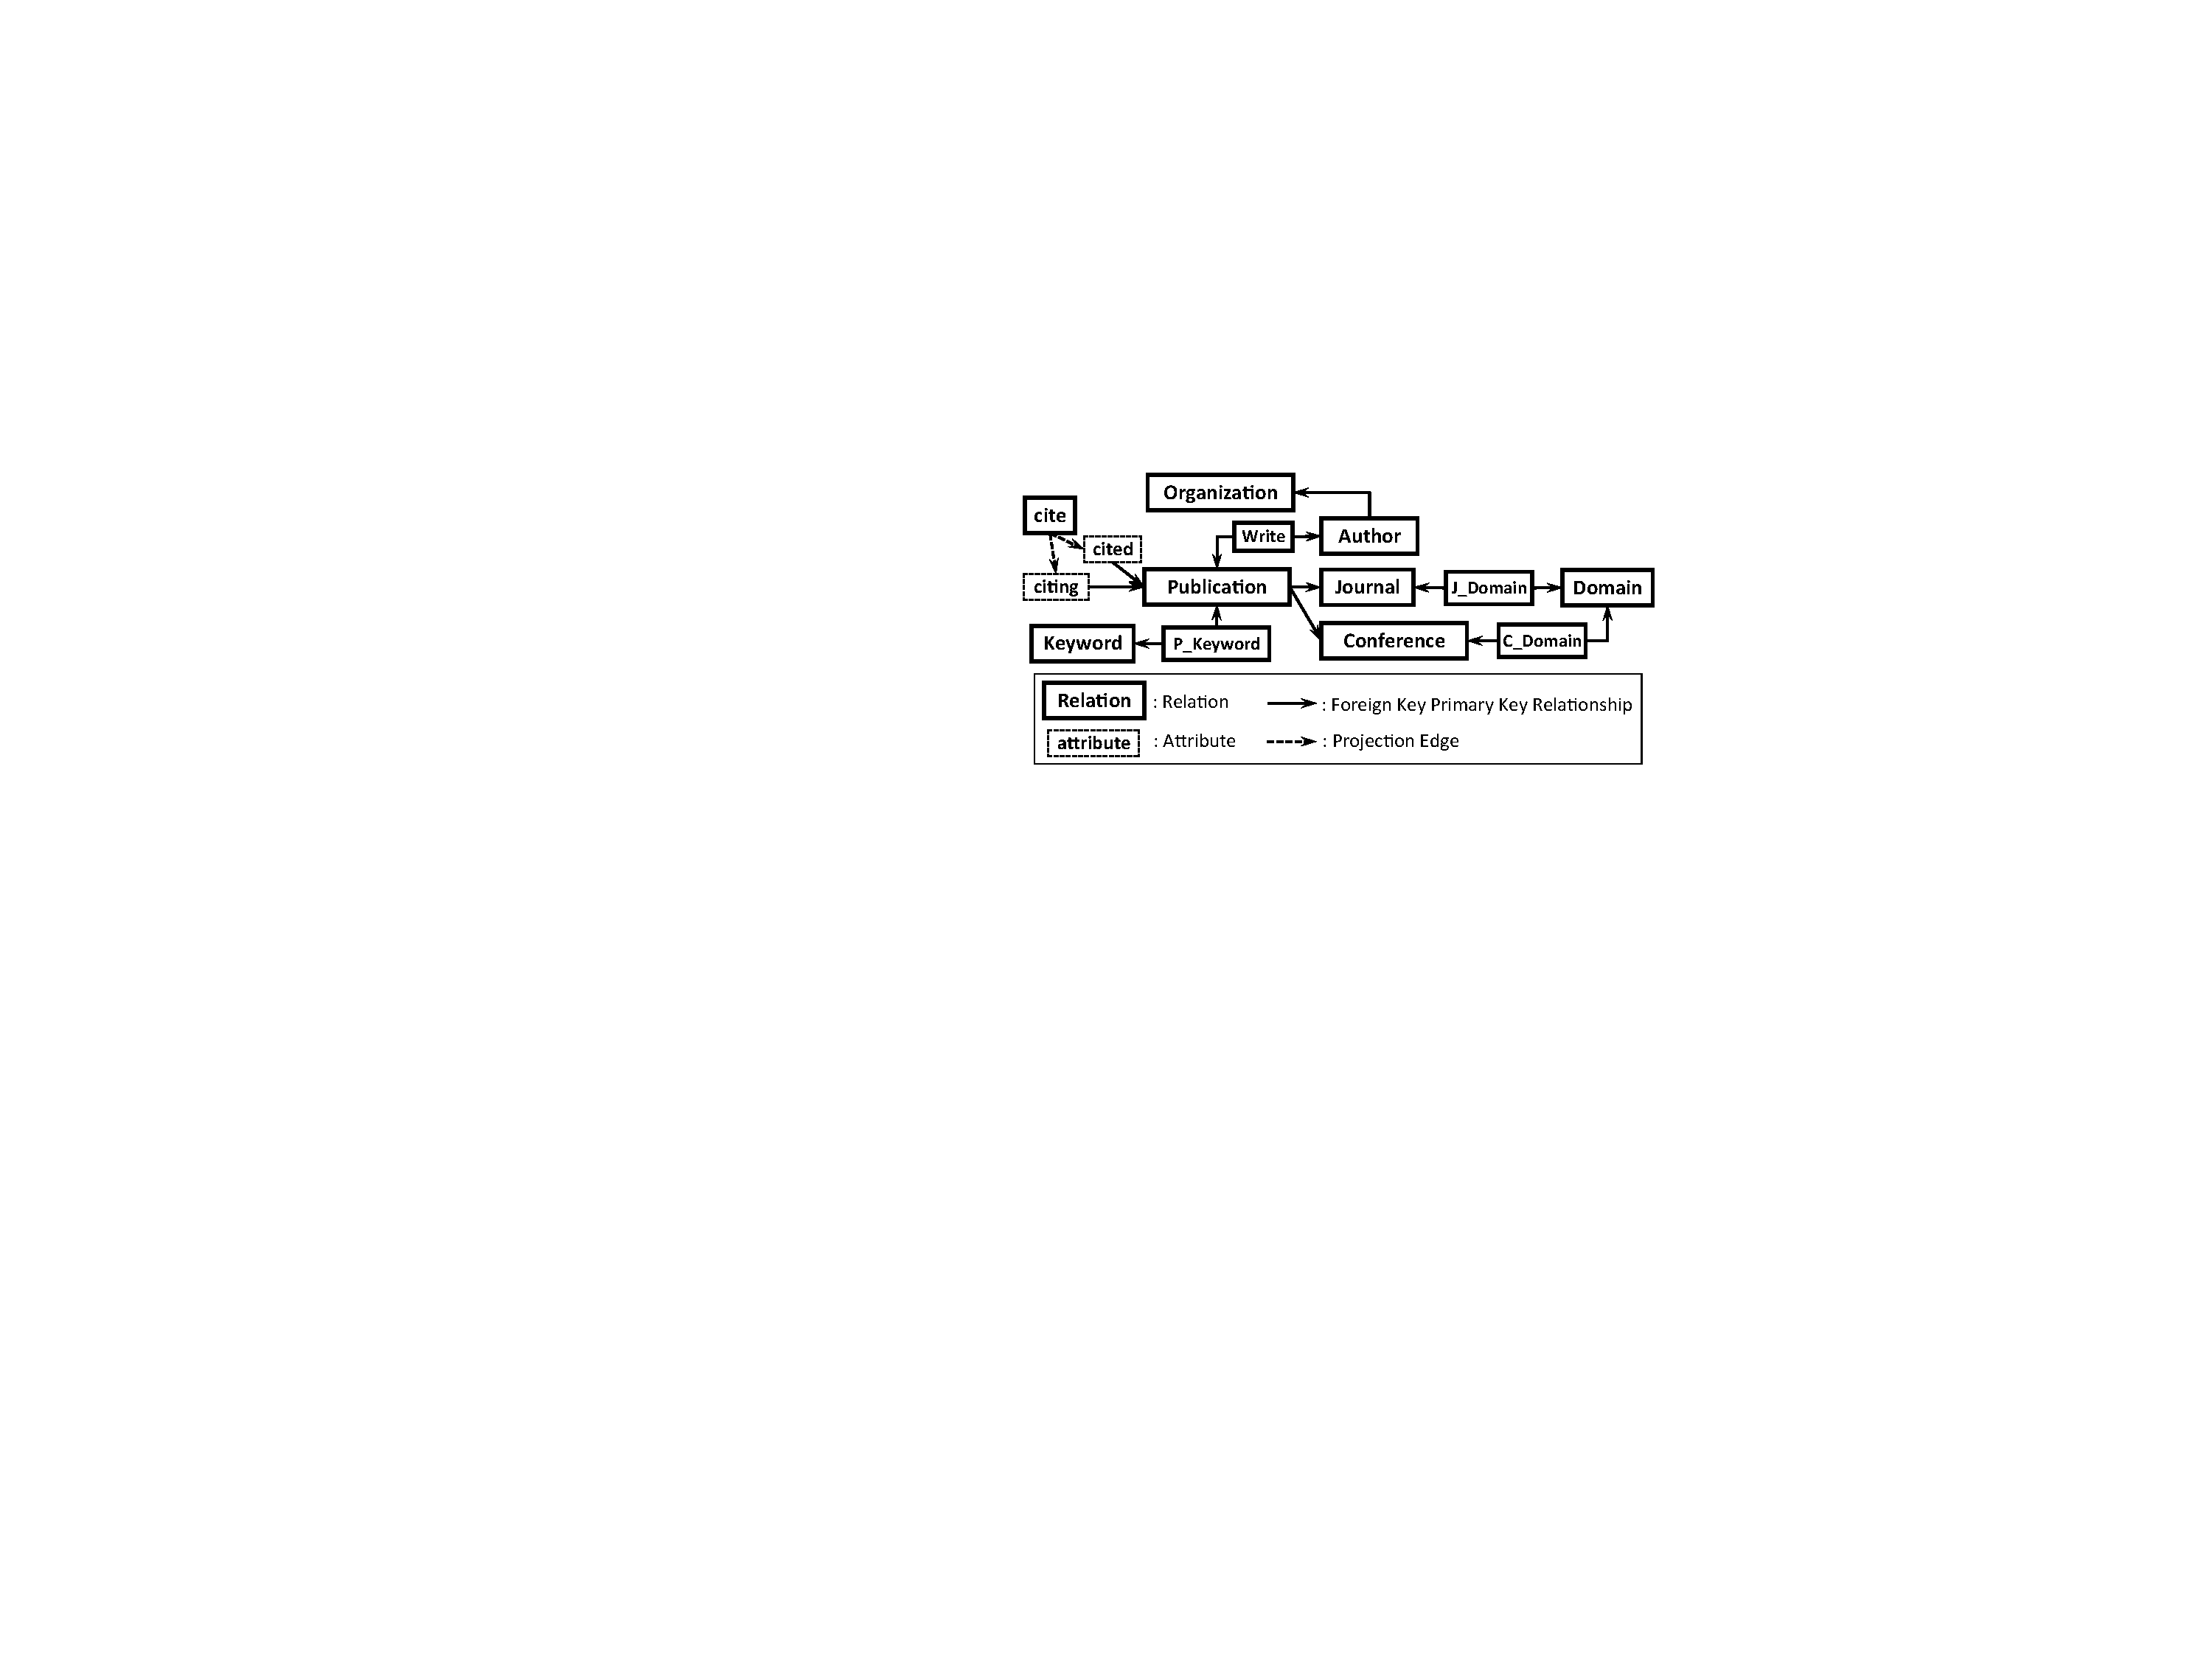
\includegraphics[width=1\linewidth]{pic/runningExample.pdf}
  \caption{A Simplified Schema Graph for Microsoft Academic Search}
  \label{fig:runningExample}
\end{figure}
\end{example}

\begin{example}
\label{example:feifeiliFirst}
When users using natural language interfaces, some of them would prefer brevity and specify queries like ``who have more papers in SIGMOD than Feifei Li".  Others might be aware that they are interacting with computers and try to specify a more completed query on purpose like ``show me the authors, in which the number of papers on SIGMOD by the author is more the number of papers on SIGMOD by Feifei Li".  Both of the two expressions might be hard for most NLIDB to process since the first one has many ambiguities while the second one is too long for most parser to parse correctly.  
\end{example}

A central challenge in building an NLIDB is the huge variability in natural language expressions: there are many ways to say the same thing, with differences possibly not only in the specific words used but even in the structure of the sentences.  In consequence, it is unlikely that a simple rule-based translator can handle this huge variation.  This sort of variability in natural language has been a central challenge in semantic parsing and machine translation for many years.  Recently, deep learning has generated much enthusiasm as being able to \emph{learn} these hidden structures.
In most of the recent works, understanding a natural language query is often modeled as a semantic parsing problem or machine translation problem, in which the translator is learned from $(NLQ, SQL)$ pairs of training examples~\cite{DBLP:conf/acl/DongL16,DBLP:journals/debu/LuLK16,DBLP:journals/cacm/Liang16,DBLP:journals/tacl/ReddyTCKDSL16}.    However, in this strategy, the potential output forms an open set, which covers all the possible semantic meaning representations that are syntactically valid.  In addition, the expressions describing the same query logic can be various.   As a result, a considerable number of training examples are needed.  While obtaining such training data may be challenging, it can at least be considered, for a specific database schema of interest.  But unlike typical semantic parsing or machine translation problems, the underlying schema of different databases often differs, which means the training set for one NLIDB cannot be applied to another NLIDB.  As a result, in real database applications, enough training data is virtually impossible to collect.  Furthermore, any learned translator will work only until the next schema update, after which additional training is required.

We observe that, given a database, the potential queries are often predictable, since the questions that can be answered is constrained by the schema and the data of the database. As such, the system does not need to support any query logic beyond that scope. Actually, the query logics needed to support are even much narrower than that can be answered by a database. Although there might be infinite number of different queries over the database, the frequently asked ones are often limited and are likely to be covered by a set of SQL templates, in which each SQL template corresponds to one query logic. Given this observation, we model the semantic coverage of an NLIDB as a set of SQL templates. The problem of understanding an NLQ is simplified as a mapping problem, which tries to map the NLQ to its corresponding SQL template. By this design, the system does not need to understand every detail of the natural language query or compose the SQL statement from the ground.  

To find the desired SQL template for the natural language query, we need to detect the similarity between them, given the possible variant of the input.  We observe that although the potential number of different expressions might be large, the expressions that are likely to be frequently used by real users are often in limited numbers of groups, in which the expression in each group are only different in stop words, word order or synonyms.  That means, for a query logic with a few different natural language expressions previously recorded, each new natural language expression describing the same query logic should be, in most cases, very similar to at least one of the previous expressions.  As such, the problem is broken down as how to effectively detect the similarity between natural language expressions and how to collect different natural language expressions for each SQL template. 

\begin{example}
Consider the query in Example~\ref{example:30} again.  When specifying this query logic, users may use other expressions.  But in most cases, the expressions they used should be very similar to one of the above two expressions.  As such, by capturing the similarity between the new coming natural language query and the two expressions, the system should be able to recognize that the expressions specifying that query logic.  As such, if we already have these two expressions, it would be easy to recognize the same query logic by comparing the new query with these two expressions.  
\end{example}

The immediate challenge would be how to capture the similarity between similar natural language expressions.  Early works like TF-IDF dealt with the stop words in a principled way but does not capture the similarity between individual synonyms.  Recent works attempt to learn a latent low-dimensional representation of sentences~\cite{DBLP:conf/icml/LeM14} from a generic corpus.  This strategy may works well in document matching.  However, in our situation, all the natural language queries are describing some query logic focusing on a narrow domain (the underlying database).  Sentences with different semantic meanings might be embedded very close to each other.  Other metrics with hyperparameters, which try to capture the complex structure of natural language, may be hard to configure, given the difficulty of gathering enough training data on the querying domain.  

As such, the metrics we present are hyperparameter free, which means they can be used even in the cases when the training examples are very limited.  Specifically, our approach leverages the recent results of word2vec~\cite{DBLP:conf/nips/MikolovSCCD13}, which embeds words to low-dimensional vectors, in which words semantically similarity to each other are close in the space.  We represent each word as low-dimensional vectors and model sentences as sets of low-dimensional vectors.  The distance between two sentences is defined as the minimum cost of traveling the words in one sentence to the words in the other sentence.  One problem in such evaluation is that the influence of common words (or even stop words) would be the same as special words.  To deal with this problem, we merge of TF-IDF with the distance computation of word vectors.  Using our metrics, the similarity between the expressions that are different in stop words, word order or synonyms is effective detected.  

At the cold start stage, we use generic metrics to capture the similarity between an natural language query and a SQL template.  After collecting some expressions, our system maps the new query to the SQL template based on the previous expressions on that template.  To collect the training data, we design an interactive communicator for the NLIDB.  Top mapped SQL templates with value instantiations are explained for the user to choose from.  Once the user make a choice, NLQ paired with the chosen SQL template is collected, which serves as the prefect training set to improve the system.  The choosing action implies the fact that the user has verified the interpretation.  As such, we could assume that most of the training examples collected in this process are correct.  In some extreme cases, a small part of the training examples collected might be incorrect matching pairs, which will disturb the mapping for the future similar queries.  As will be discussed, our system prefers to rank a SQL template higher if it is associated with more previous NLQs showing high similarity with the new query.  In such design, the desired SQL template are likely to be mapped, as long as most of the relevant training examples are correct.  

Besides finding the desired template, the slots in the template must be instantiated correctly to generate the correct SQL statement. As such, the ambiguities at entity level need also to be fixed. The identification for an entity used in natural language scenarios and stored in a database are often different. In a database, keys are defined to distinguish entities from each other while in natural language scenarios, the identifications are often the text values. However, text values stored in the database may be very similar or even exactly the same, even if they are corresponding to different entities. Consider Example~\ref{example:feifeiliFirst} again.  There might be more than one authors in the database named Feifei Li and have papers in SIGMOD. The system needs to figure out which one is the desired from the user.  In our system, we model the database as a data graph. The nodes that are connected by many paths are considered strongly connected. When disambiguating the entities, we prefer to choose the combination that is strongly connected to each other, in which the context in both the NLQ and the data graph are taken into account. 

Putting the ideas together, we propose a framework for building NLIDBs.  The NLIDBs constructed could work even in the cases when no training data is available.  It collects the training data through real usage and benefits from it accordingly.  The intellectual contributions of this paper are as follows: 
\begin{enumerate}
  \item The problem of natural language interpretation is modeled as finding its corresponding SQL template and instantiating the template.  We present a generic metric to evaluate the relevance between NLQ and SQL template, which could work even in the cases when no training examples are available.  
   \item We present metrics that are hyperparameter free, which could effectively detect the similarity between natural language expressions describing the same query logic, even in the cases when the training examples are limited.  
  \item We provide strategies for matching the entities mentioned in the NLQ to that stored in the database, in which the matching considers the context of both the NLQ and the data structure of the database. 
  \item Interactive communications are designed, in which multiple interpretations with explanations are returned for the user to choose from.  This design could improve the recall and reliability of the NLIDB and most importantly, the user behavior data it collects could be used as training data to improve the performance of the system. 
\end{enumerate}

The remaining parts of the paper are organized as follows.  In Section~\ref{sec:overview}, we overview our strategy in disambiguation of natural language queries.  Section~\ref{sec:queryMapping} discusses the mapping from an NLQ to the SQL templates.  We provide methods to resolve the ambiguities at entity level in Section~\ref{sec:entityMapping}.  The system architecute is presented in Section~\ref{sec:architecture}.  In Section~\ref{sec:experiments}, our system is evaluated experimentally.  We discuss related works in Section~\ref{sec:relatedWork}. In Section~\ref{sec:conclusion}, we draw conclusions and point to future work.

\section{Preliminary}
\label{sec:overview}
The input to our system is a natural language query whose semantic meaning may involve comparisons, aggregations, various types of joins and nestings, among other things.  The semantic coverage of our system is a set of predefined SQL templates.  Given a natural language query, by mapping it to the correct SQL template and instantiating the values, our system translates the natural language query into the desired SQL statement and evaluates it against an RDBMS.  In this section, we first overview our solution and then define the SQL template.  

\subsection{Semantic Coverage}
The problem we attempt to address is to translate a natural language query (NLQ) to a SQL statement.  This problem would be difficult if it is modeled as a semantic parsing problem or machine translation problem, like most previous works did.  The fundamental problem is that natural language queries are inherently ambiguous.  Even a grammatically correct natural language sentence may contain ambiguities, from both the perspective of natural language processing and the perspective of database schema matching.  Moreover, naive users often use informal expressions and prefer brevity to logical precision.  These challenges make it difficult to understand the query and compose the correct SQL statement from the scratch.  
\begin{example}
\label{example:semanticCoverage}
Consider a simple query ``papers with 5000 citations" on the database shown in Figure~\ref{fig:runningExample}.  Many ambiguities exist.  For example, in this query, ``5000 citations" is more likely to mean ``more than 5000 citations".  Also, when generating the join path between ``paper" and ``citation", it is hard to figure out the direction of ``citing" and ``cited", in which one of them means citation while the other means reference.  Due to these ambiguities, the query can correspond to four SQL statements with semantics that are different, leading to different query results.
\end{example}

In our strategy, we would like to simplify the problem.  First, given a database, we do not need to understand any natural language query beyond the scope of the information that can be provided by the database.  Second, we only need to support the query logics that are semantically meaningful, which are only a very small subset of syntactically valid ones.  Consider the Example~\ref{example:semanticCoverage} again.  All the four interpretations are syntactically valid but only the correct interpretation out of the four interpretations are semantically meaningful, since users are not likely to query a paper with an exact number of citation or a paper with more than a number of references.  By not supporting the unnecessary query logics, many ambiguities are removed naturally.  Based on this observation, the task of interpreting a natural language query would be much easier if the system is designed to support only the necessary query logics that are likely to be frequently asked.  As such, in our system, we would like to define the semantic coverage of an NLIDB as a set of necessary SQL templates, which can either be enumerated by experts or learned from a query log of SQL queries.  Then the task of natural language interpretation is simplified to recognizing the desired SQL template and filling the slots in the template.  

\subsection{SQL Template}
\label{subsec:SQLTemplate}
Often, two queries are said to have the same SQL template if they have the same SQL structure (SQL keywords, relations, attributes, aggregation functions, operators, nestings), even though constants in the query have different values.  A SQL template is used to represent such SQL queries by replacing the specific values in the SQL statement with slots.  In some cases, two SQL templates may have exactly the same query logic.  In such cases, these SQL templates are merged, in which each original SQL template serves as an expression of the template and the one that can be evaluated most efficiently over an RDBMS is considered as the default expression of the template.  
\begin{example}
\label{example:example1}
The SQL template corresponding to ``authors who have more than 30 papers, in which each of these papers have more than 30 citations" is shown in Figure~\ref{fig:sampleTemplate}.  This SQL template may have other expressions.  For example, the part corresponding to the ``citation of each paper" can be written as a subquery, which has the exactly the same query logic but evaluated less efficiently.  As such, the expression shown in Figure~\ref{fig:sampleTemplate} is used as the default expression for the SQL template.  
\begin{figure}[h]
\center

\includegraphics[width=1\linewidth]{pic/sampleTemplate.pdf}
\caption{Sample SQL Template.}
\label{fig:sampleTemplate}
\end{figure}
\end{example}

So the question is how to map the input natural language query to the SQL templates.  Search engines also deal with a mapping problem, which maps a set of keywords to documents, and receive great industry success.  As we think about mapping from a natural language query to the SQL templates, it is worthwhile to draw inspiration from search engines, and to see how they do the ranking.  At the early stage of search engines, the mapping is mainly based on metrics combined of relevance (e.g. using TF-IDF) and the importance of webpages (e.g. estimated using PageRank)~\cite{Page99thepagerank}.  After collecting training examples in the form of (keywords, page clicked), the ranking is improved with learning to rank frameworks~\cite{DBLP:books/daglib/0027504}.  In our system, we adopts this general design, we start from using metrics to evaluate the relevance between a natural language query and SQL templates.  After training examples are collected, the mapping is improved accordingly. 

\paragraph*{Training Example}  The training examples are in the form of pairs of $(NLQ, SQL)$.  In preprocessing, a SQL query is transformed to SQL template.  Similarly, the natural language query is also preprocessed to a natural language template by replacing the values with slots.  For example, the natural language query ``citations for `constructing an NLIDB' by others" is preprocessed to ``citations for \$publication by others". 

\section{Query Mapping}
\label{sec:queryMapping}
In this section, we interpret the whole query by mapping it to the SQL templates.  Given a natural language query $\mathit{NLQ}$ and a SQL template $T$, we measure the relevance between them based on two intuitions.  First, if the information specified in $\mathit{NLQ}$ and $T$ are heavily overlapped, it is likely that $T$ is the desired SQL template of $\mathit{NLQ}$.  This kind of relevance could be measured even in the cases when there are no training examples available.  This intuition will be quantified in Section~\ref{subsec:overlap}.  Second, if a previous query $\mathit{NLQ'}$ paired with $T$ exist in the training set and the new coming $\mathit{NLQ}$ shows high similarity with query $\mathit{NLQ'}$, it is very likely that $\mathit{NLQ}$ should be mapped to $T$.  Measurements are provided to evaluate the similarity between the natural language queries in Section~\ref{subsec:training}. In Section~\ref{subsec:mappingRelevance}, we map the natural language query to the templates based on both the SQL expression and the training examples.  

\subsection{Information Overlap}
\label{subsec:overlap}
After the tokenization, which will be discussed in detail in the next section, the natural language query is represented as a set of the mapped SQL components.  Given the fact that trivial nodes are not considered, most of the information specified in \emph{NLQ} should be contained by the SQL template $T$, if it is relevant to \emph{NLQ}.  Reciprocally, one would think most of the information in $T$ should also be contained in \emph{NLQ}.  However, natural language queries tend to be brief and often leave out things that ``can be understood".  Furthermore, natural language queries typically do not include schema-specific constructs such as FK-PK join paths, which are often by-products of normalization.  So, in the reciprocal direction, we expect that most of the {\em major} information in $T$ should also be contained in \emph{NLQ}, according to a definition of {\em major} that we provide in the next paragraph.  Putting these ideas together, \emph{NLQ} is considered relevant to $T$ if (a) the information in \emph{NLQ} is contained by $T$, and (b) the major information in $T$ is specified in \emph{NLQ}.  
\begin{example}
For the query of ``authors focusing on database usability" on the database in Figure~\ref{fig:runningExample}, its corresponding SQL template has a join path from ``author" to ``keyword" through ``write" and ``paper".  In this SQL template, ``author" is the element that are returned, ``keyword" has a value constraint of ``database usability", which means both of them should be mentioned by the user.  In contrast, ``write" and ``paper" are in the middle of the join path, which is likely to be omitted in a natural language query. 
\end{example}

In our sytem, we capture intuition (a) by computing the raio between $\mathit{|Info(NLQ) \cap Info(T)|}$ and $\mathit{|Info(NLQ)|}$, in which $\mathit{Info(NLQ)}$ is the set of mapped SQL components of the phrases in \emph{NLQ} and $\mathit{Info(T)}$ is the set of the SQL components in $T$.  This ratio measures how much proportion of the information specifies in $NLQ$ are also specified in $T$.  

Similarly, the intuition (b) is captured as the ratio between $\mathit{|MInfo(NLQ) \cap MInfo(T)|}$ and $\mathit{|MInfo(T)|}$, in which $\mathit{MInfo(NLQ)}$ is the set of nodes in \emph{NLQ}, while $\mathit{MInfo(T)}$ is all the \emph{major nodes} in the SQL template $T$.  The major nodes are the nodes whose information is important and unlikely to be omitted by the user.  For example, a schema element that is returned or has a value constraint is considered as a major node, since it is not likely to be omitted by the user, while the schema element that serves only as a middle node in the join path is not considered as  a major node, since it is often implicit in the user's query.  

In our system, the information overlap between a natural language query and a SQL template is defined as the average of the two ratios mentioned above. 

\subsection{Semantic Distance between Queries}
\label{subsec:training}
To evaluate the similarity between sentences, early works often represent sentences as bags of words/$n$-grams or strings, and use metrics like Jaccard Coefficient or edit distance to evaluate the similarity between them.  The limitation is that in these methods, the semantic similarity between different words is not captured.  Recently, a stream of researches attempt to solve this problem by learning a latent low-dimensional representation of sentences and work well in document matching~\cite{DBLP:conf/icml/LeM14}.  However, in our situation, all the natural language queries are describing some query logic focusing on a narrow domain (the underlying database).  In such situation, if trained from a generic corpus, the low-dimensional space may not be able to distinguish the natural language queries with slightly different query logics, in which natural language queries may too close to each other in the low-dimension space even in the cases when they correspond to different SQL template.  The most straightforward  way is to train the model using the data in the querying domain.  However, in most situations, it is almost impossible to obtain large numbers of training examples over the domain of the specific querying database.  

In this section we introduce new metrics for the distance between natural language sentences.  The metrics we designed are hyper-parameter free, which means they can be used even in the cases when the training examples are very limited.  Specifically, our approach leverages the recent results of word2vec~\cite{DBLP:conf/nips/MikolovSCCD13}, which embeds words to low-dimensional vectors, in which words semantically similarity to each other are close in the space.  The authors demonstrate that semantic relationships are often preserved in vector operations on word vectors, such as vec(Picasso) - vec(painter) $\approx$ vec(Einstein) - vec(scientist) and vec(sushi) - vec(Japan)  $\approx$ vec(bratwurst) - vec(Germany)~\cite{DBLP:conf/nips/MikolovSCCD13}.  Follows~\cite{DBLP:conf/icml/KusnerGGW15}, our metrics utilize this property of word2vec embeddings to capture the distance between individual words.  We represent each word as low-dimensional vectors and model sentences as sets of low-dimensional vectors.  The distance between two sentences is defined as the minimum cost of traveling the words in one sentence to the words in the other sentence.  

\begin{example}
Consider a natural language query ``authors with h-index over 40" ($\mathit{NLQ}$).  It is very hard to map $\mathit{NLQ}$ to the SQL template shown in Figure~\ref{fig:sampleTemplate} directly.  However, if we have a training example, which is ``whose h-index is larger than 35" ($\mathit{NLQ'}$) paired with the SQL template in Figuree~\ref{fig:sampleTemplate}, capturing the similarity between $\mathit{NLQ}$ and $\mathit{NLQ'}$ could help the system to understand $\mathit{NLQ}$.  We adopt the basic idea in~\cite{DBLP:conf/icml/KusnerGGW15}.  All words of both queries are embedded into a word2vec space.  The distance between the two documents is the minimum cumulative distance that all words in $\mathit{NLQ}$ need to travel to exactly match $\mathit{NLQ'}$.  
\begin{figure}[h]
\center
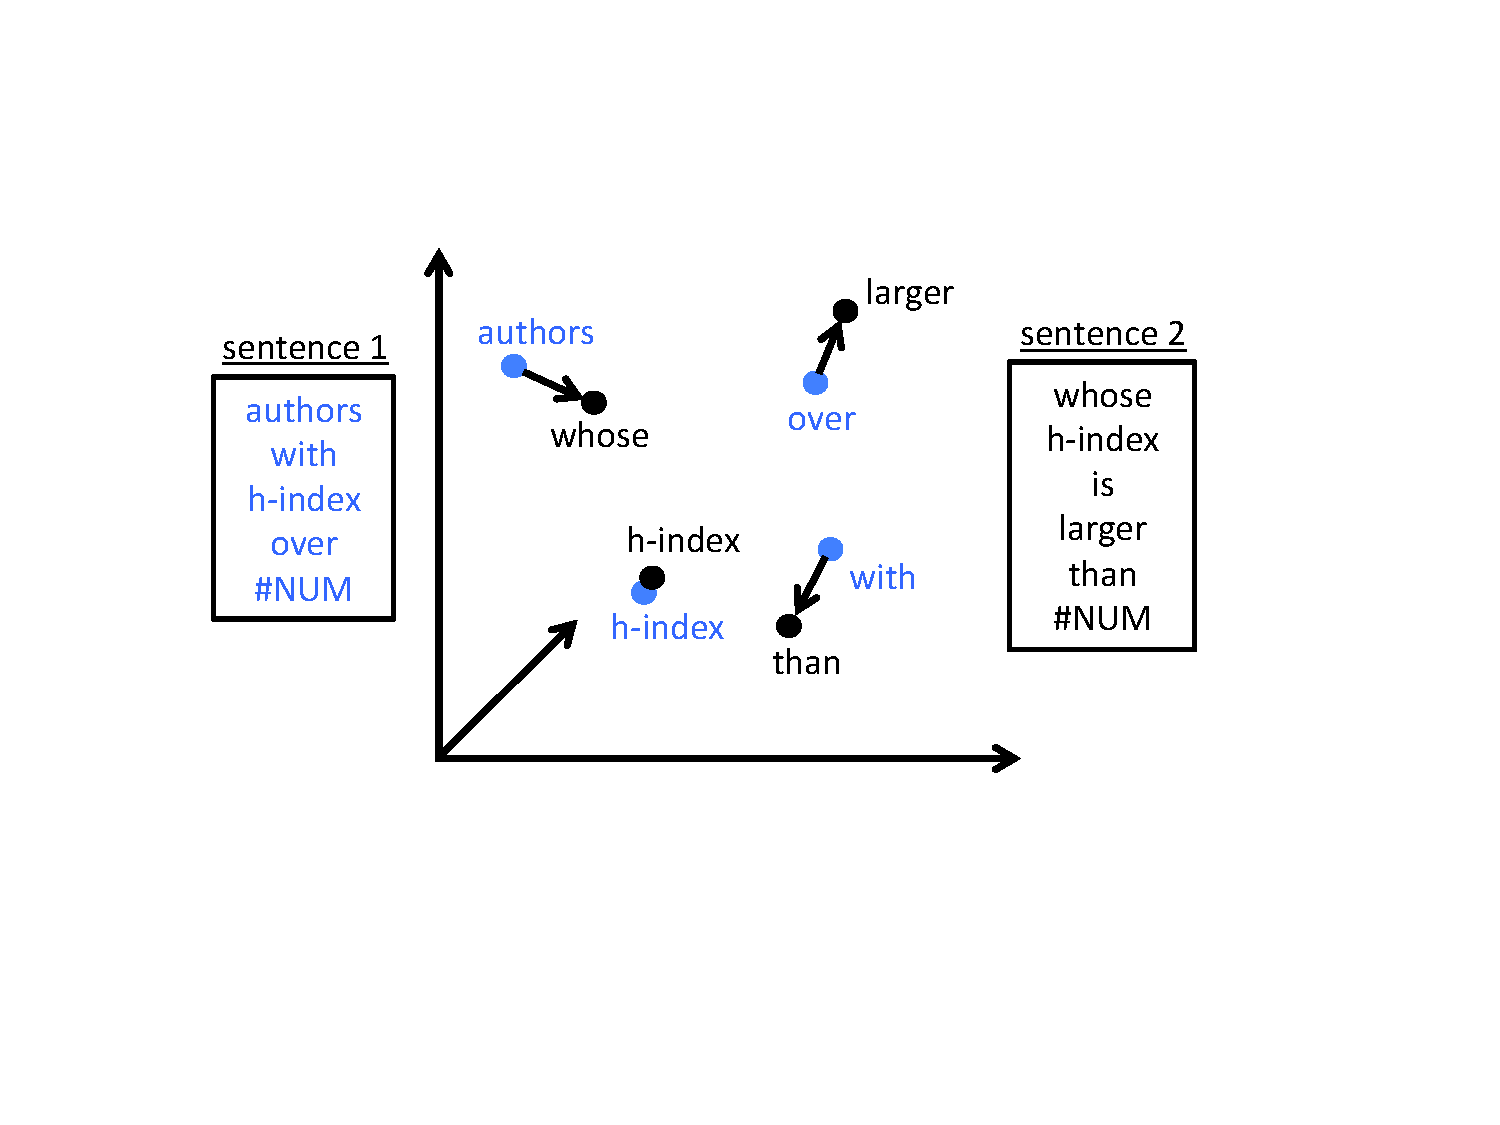
\includegraphics[width=0.9\linewidth]{pic/word2vec.pdf}
\caption{Word to Vector Embedding.}
\label{fig:sampleTemplate}
\end{figure}
\end{example}

The major problem in the Word Mover's Distance provided in~\cite{DBLP:conf/icml/KusnerGGW15} is that common words and rare words have the same impact in the distance evaluation.  Intuitively, the fact that a very rare word in one sentence cannot find similar words in the other sentence should cause a large distance for the two sentences.  In contrast, if two sentences only differ in the semantic of some common words (or even stop words), they should not be assigned a large distance.  As such, we take the term frequency-inverse document frequency (TF-IDF) of each word into account, in which the influence of rare words is augmented while influence of common words are reduced.  

\paragraph*{Word Travel Cost}
Our goal is to incorporate the semantic similarity between individual word pairs (e.g. coauthor and collaborator) into the distance metric between two query sentences.  One such measure of word distance is naturally provided by their Euclidean distance in the embedding space.  More precisely, the semantic distance between word $w$ and word $w'$ becomes $||vec(w) - vec(w')||$.  In addition, when traveling one word to another word, the cost is defined as $\mathit{tfidf(w) * ||vec(w) - vec(w')||}$.  

\paragraph*{Word Travel Cost from Sentence to Sentence}
The travel cost from one word to another is a natural building block to create a distance between two sentences.  Let $\mathit{NLQ}$ and $\mathit{NLQ'}$ be two natural language sentences.  The word travel cost from $\mathit{NLQ}$ to $\mathit{NLQ'}$ is defined as the minimum cumulative cost required to travel each word in $\mathit{NLQ}$ to the words in $\mathit{NLQ'}$.  

\paragraph*{Sentence Travel Distance}
Given two natural language queries $NLQ$ and $NLQ'$, the sentence travel distance between them is defined as the average of the word travel cost from $\mathit{NLQ}$ to $\mathit{NLQ'}$ and the word travel cost from $\mathit{NLQ'}$ to $\mathit{NLQ}$.  We denote it as $\mathit{Travel(NLQ, NLQ')}$.  

\subsection{Template Mapping}
\label{subsec:mappingRelevance}
As mentioned in Section~\ref{subsec:SQLTemplate}, a query logic may be expressed in different SQL expressions.  In such cases, the SQL templates with the same query logic are merged into one SQL template, in which each original SQL template serves as an SQL expression of the template.  Also, given a set of training examples, there might be multiple natural language expressions corresponding to the same SQL template.  As such, in our system, a SQL template is associated with $m$ SQL expressions and $n$ natural language expressions, in which $m$ is at least 0 and $n$ grows with the gathering of training examples for that template.  Here we denote all the know expressions (including SQL expressions and natural language expressions) for the template $T$ as $\mathit{Expression(T)}$. 

When specified in natural language, the same query logic might have very different expressions.  As such, when deciding whether a natural language query $\mathit{NLQ}$ should be mapped to a SQL template $T$, the fact that $\mathit{NLQ}$ shows high similarity with some expressions in $\mathit{Expression(T)}$ often means a lot.  In contrast, the fact that $\mathit{NLQ}$ shows low similarity with some expressions in $\mathit{Expression(T)}$ does not mean that they should not match.  So, when evaluating the probability of matching $\mathit{NLQ}$ with $T$, we focusing only on the old expressions showing high similarity with $\mathit{NLQ}$ and see how many of them are coming from $Expression(T)$.  

In our system, an natural language (resp. SQL) expression is considered to describe the same query logic with the natural language query $\mathit{NLQ}$ when their distance (resp. similarity) is below (resp. above) a threshold.  Based on this assumption, the probability that $\mathit{NLQ}$ should be mapped to $T$ can be computed as the ratio of the number of expressions in $Expression(T)$ showing high similarity with $\mathit{NLQ}$ over the number of expressions of all the templates showing high similarity with $\mathit{NLQ}$.  

\section{Entity Disambiguation}
\label{sec:entityMapping}
Given an online natural language query, before finding its corresponding SQL templates in the semantic coverage, we first interpret its words/phrases by mapping them to the database elements (SQL keywords, schema elements and database values).  Such phrases can be further divided into different types as shown in Figure~\ref{fig:nodeType}, according to the type of database elements they mapped to.  The identification of select phrase, operator phrase, function phrase, quantifier phrase and logic phrase is independent of the database being queried.  Following~\cite{DBLP:journals/tods/LiYJ07,DBLP:journals/pvldb/LiJ14}, we enumerate sets of phrases as the database independent lexicon to identify these five types of phrases.  

\begin{figure}
  \center
  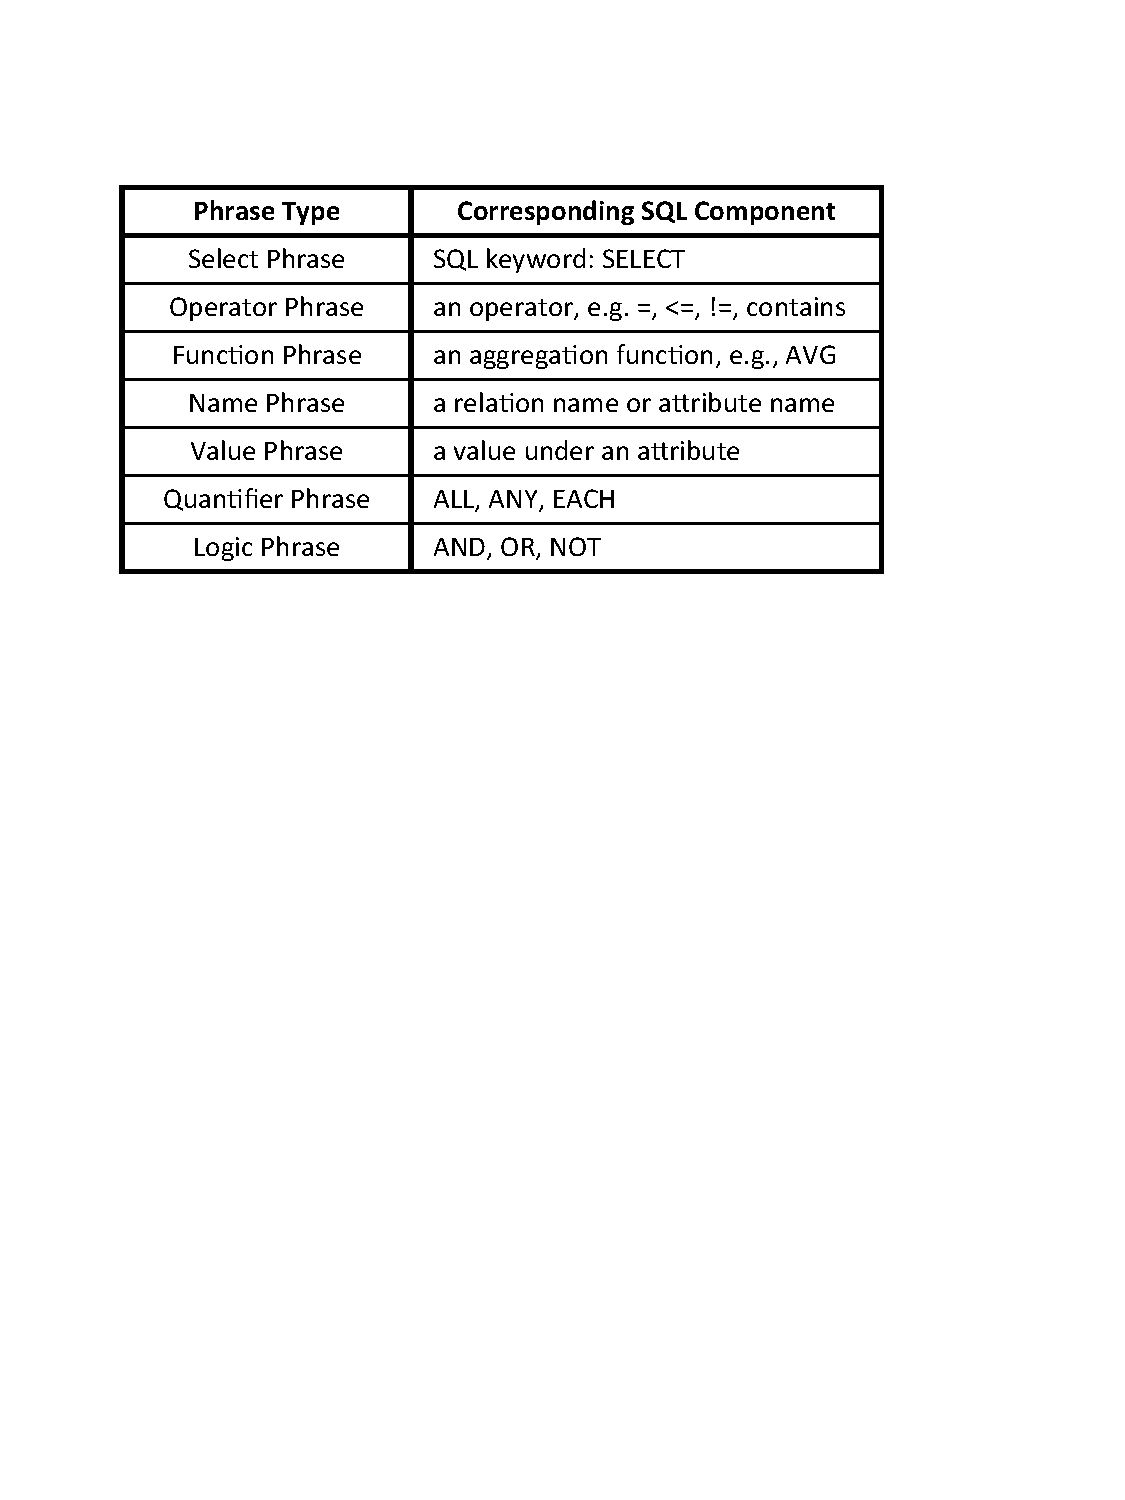
\includegraphics[width=0.85\linewidth]{pic/nodeType.pdf}
  \caption{Different Types of Phrases.}
  \label{fig:nodeType}
\end{figure}

In this process, the major challenge is the matching between the entities mentioned in natural language query and that stored in the database. The problem comes from the fact that the identification for an entity in a natural language description and that stored in a database are often different. In natural language query, users often mention an entity by its names, while in the database, keys are defined to distinguish entities from each other. Often, the users are not able to specify the exact name of the entity that stored in the database (e.g. the title of a paper). Also, many different entities in the database may have similar or even exactly the same names (e.g. names of authors). As a result, approximate matching is necessary but the matching considering only spelling is not enough. The system must figure out which entity is the desired one, given the phrases specified by the user and that stored in the database.

We notice that there may be more than one entities specified in the natural language query.  In that case, the fact that they are mentioned in one query means they are related to each other.  When matching them with the entities in the database, we prefer to choose the mapped entities are also strongly ``related" in the database.  Also, we notice that the important entities are often more likely to be queried.  So when we would also like to capture the importance of entities in the mapping.   
\begin{example}
Consider the query in Example~\ref{example:feifeiliFirst}.  There are many authors in the database named Feifei Li and several conferences/journals have names contained SIGMOD.  If one of the Feifei Li has many papers in one of the conferences/journals, it is very likely that this combination would be the desired one.  
\end{example}

In this section, we capture the intuitions of ``related" and ``importance" in a unified way.  To facilitate that, the database is modeled as data graph.  
\begin{definition}[Data Graph]
The data graph is a undirected graph, $G$ = $(V, E)$ with node set $V$ and edge set $E$, where nodes in $V$ are tuples in the database.  There exists an edge between node $v_1$ and node $v_2$ if their corresponding relations have a foreign key to primary key relationship, and the foreign key of $v_1$ equals to the primary key of $v_2$.
\end{definition}

\begin{example}
\label{example:graph}
Consider the bibliographic database in Figure~\ref{fig:runningExample} again.  The whole database is modeled as a data graph, in which each publication, author, organization, conference, journal, keyword and domain is modeled as a node.  There are too many kinds of edges in the database and we take the edges related to a publication as an example.  There is an edge between a publication and its authors, its published journal or conference, its keywords, its references and its citations.  
\end{example}

\begin{definition}[Match]
Let $k$ be an entity phrase specified in the natural language query, $m$ be a tuple in the database, and $sim(k, m)$ be a similarity metric between $k$ and $m$.  Given a threshold $\tau$, $m$ is called a match of $k$ when $sim(k, m)$ $\geq$ $\tau$.  We use $M_k$to denote all the matches of $k$.  
\end{definition}

\begin{definition}[Match Combination]
Let $K$ = \{$k_1$, ..., $k_n$\} be the $n$ entity phrases specified in the natural language query, $M_{ki}$ be the set of all the matches of $k_i$, the set of match combination $M_K$ is defined as \{$m_{k1}$, ..., $m_{kn}$ $|$ $m_{ki}$ $\in$ $M_{ki}$ $\land$ $1$ $\leq$ $i$ $\leq$ $n$\} is called a match combination of $K$.  
\end{definition}

In the query mentioned in Example~\ref{example:feifeiliFirst}, Feifei Li and SIGMOD are the two entity phrases.  Suppose that the Professor Feifei Li in University of Utah and the Professor Fei-fei Li in Stanford University are the two matches of entity phrase Feifei Li, and the SIGMOD conference and SIGMOD Record are the two matches of the entity phrase SIGMOD.  These two ambiguities would make up four match combinations.  

\begin{definition}[Joining Network of Tuples (JNT)]
Let $G(V, E)$ be the data graph, $K$ be the set of entity phrases and $m_K$ be a match combination of $K$.  $J(V', E')$ is called a Joining Network of Tuples (JNT) of $m_P$ when $J(V', E')$ is an acyclic subgraph of $G(V, E)$ and $V'$ contains all the tuples in $m_P$, and each end node is in $m_P$.  
\end{definition}

\begin{definition}[Combination Appearance]
Given a match combination $M$ and a join path length threshold $L$, the size of the $JNTs$ of $M$ within length $L$ is defined as its match combination appearance.  We denote it as A(M).   
\end{definition}

Consider again the query in Example~\ref{example:FeifeiLi} and the database in Figure~\ref{fig:runningExample}.  If the length threshold for the join path is set as 2, then the number of papers by each match combination of Feifei Li and SIGMOD is the combination appearance.  

Given the concept of combination appearance for each match combination, the probability that a combination $M$ is the desired combination is computed as the ratio between the combination appearance of $M$ and the total combination appearances of all the match combinations.  We denote this ratio as $P(M)$.  

\begin{figure}
  \center
  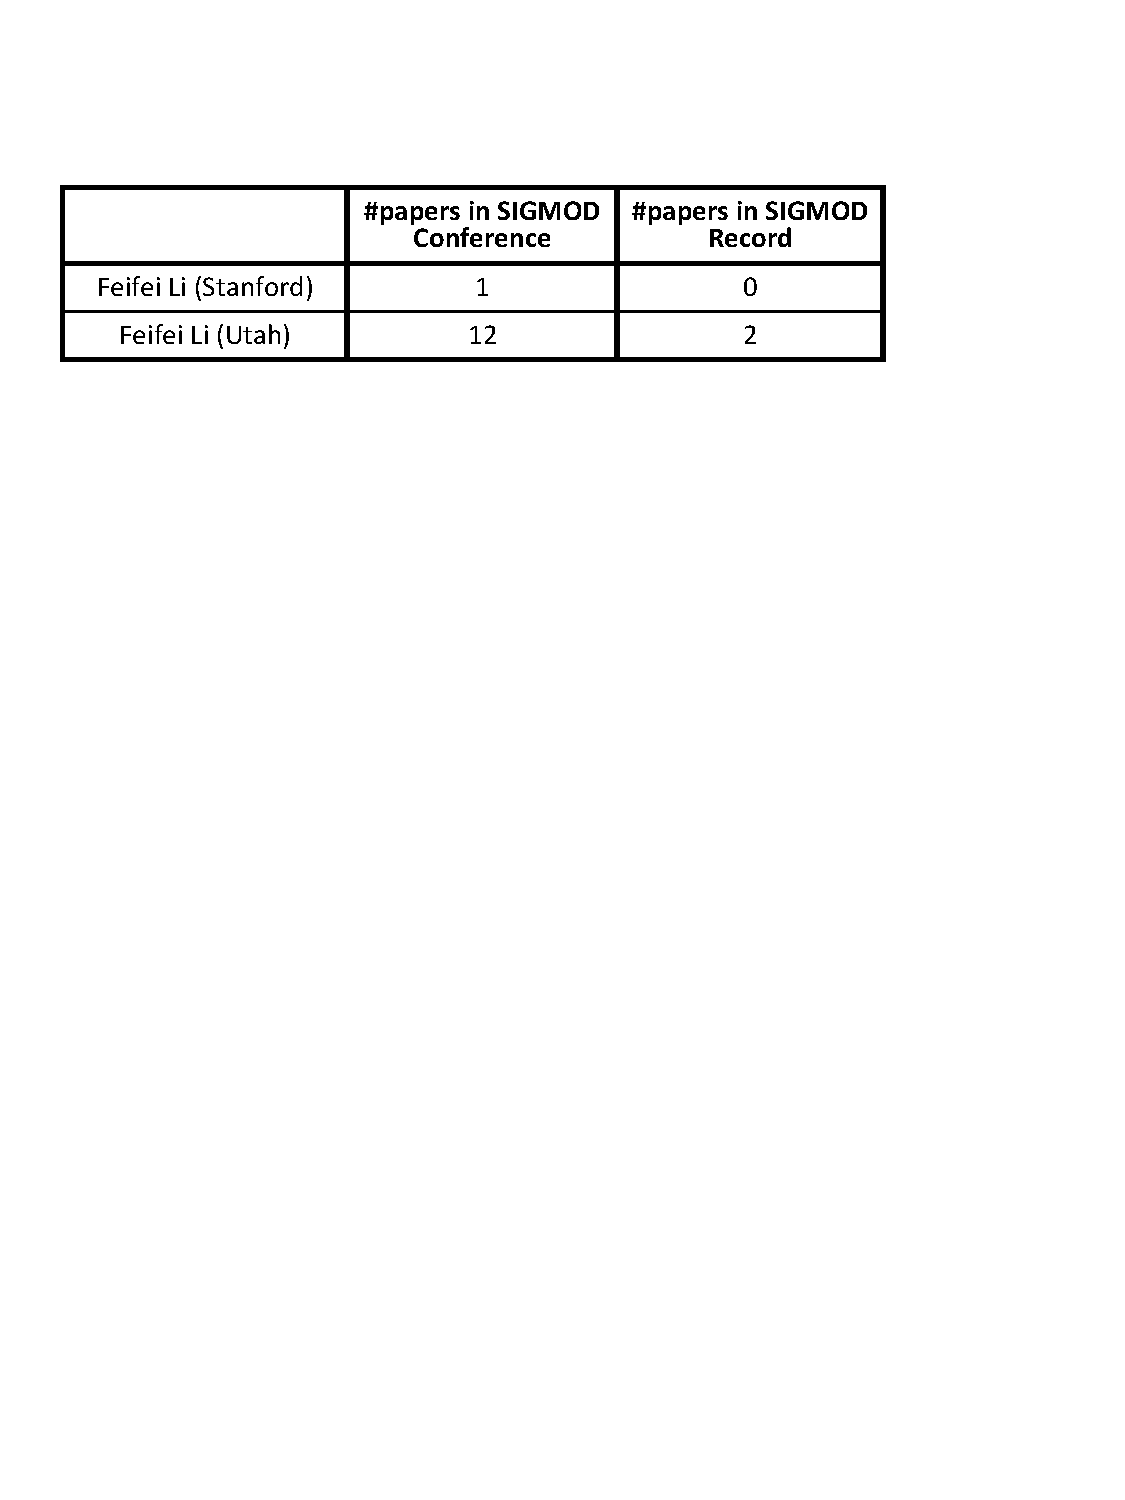
\includegraphics[width=0.9\linewidth]{pic/feifeili.pdf}
  \caption{A Simplified Schema Graph for Microsoft Academic Search}
  \label{fig:paperfeifeili}
\end{figure}

\begin{figure*}
  \center
  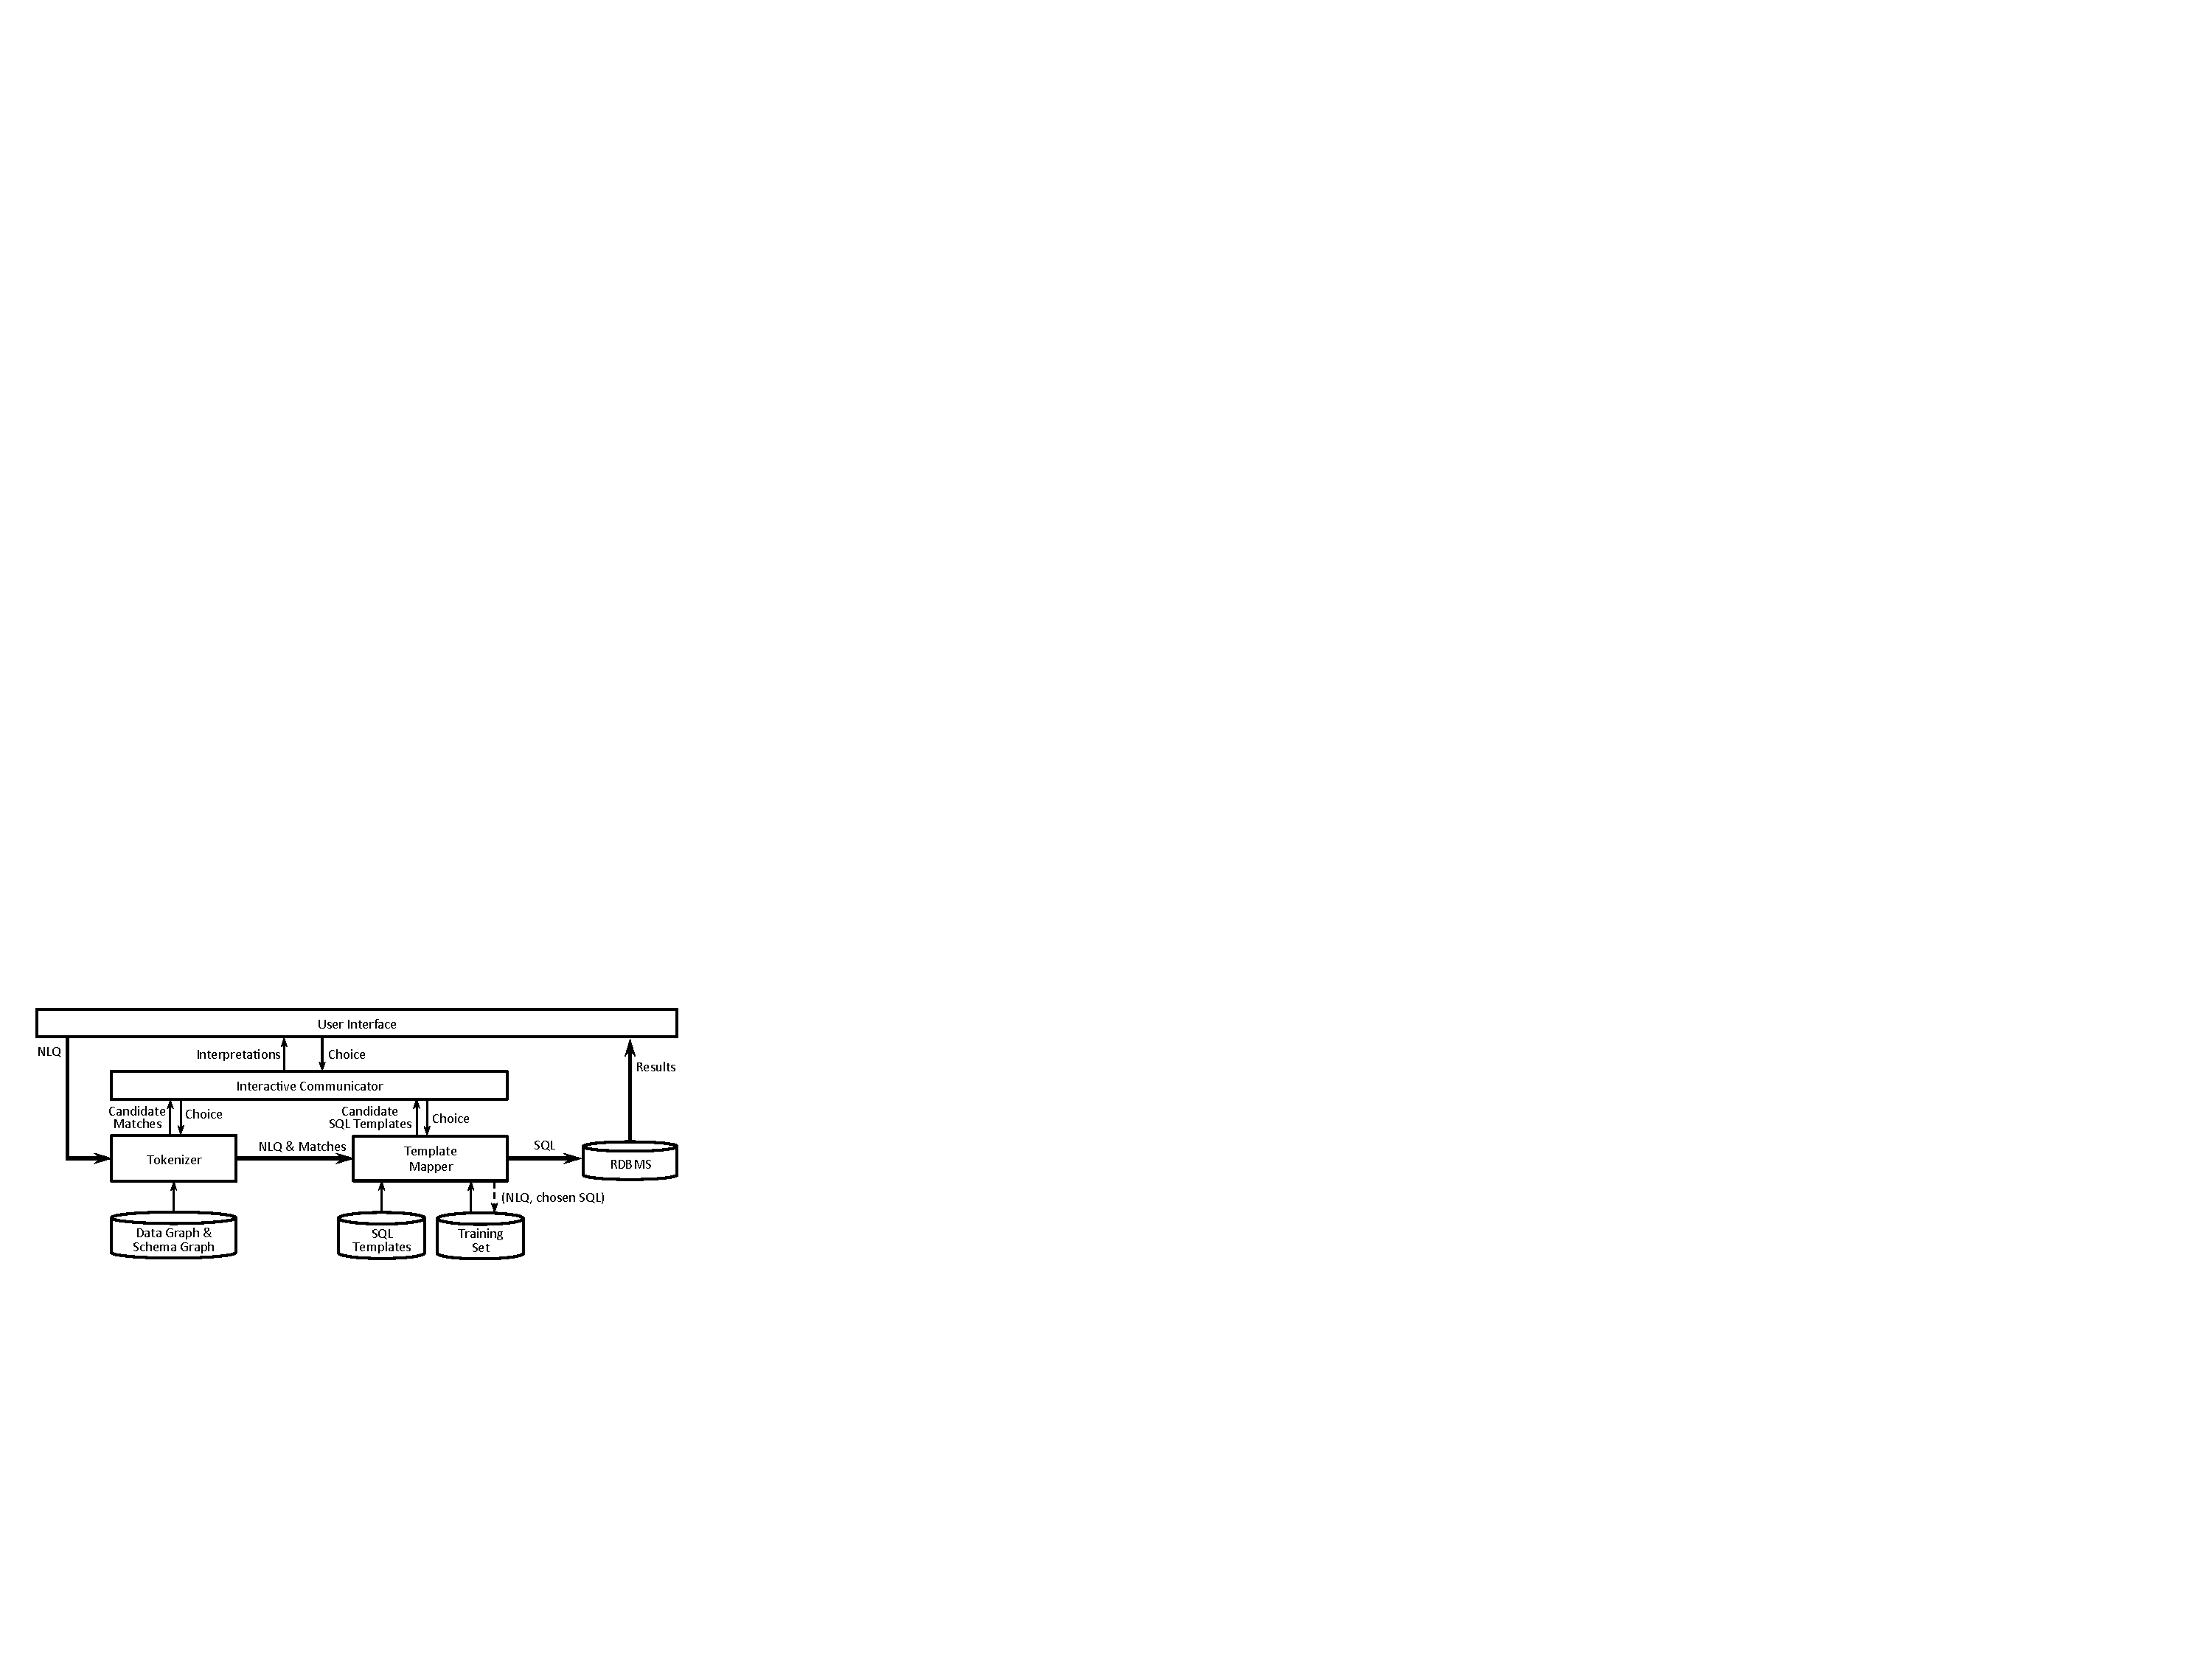
\includegraphics[width=0.8\linewidth]{pic/systemArchitecture.pdf}
  \caption{System Architecture.}
  \label{fig:systemArchitecture}
\end{figure*}

\begin{example}
\label{example:appearance}
Consider the Example~\ref{example:FeifeiLi} again.  Assume that the number of papers by each Feifei Li in SIGMOD conference/Record is the number shown in Figure~\ref{fig:paperfeifeili}, in which each number is the combination appearance if we set the length threshold as 2.  Then the probability that Feifei Li mentioned is the Professor in Utah and SIGMOD corresponds to SIGMOD Conference is 12/15 = 0.75.  The probability of other combinations can be computed in the same way.  
\end{example}

The final overall matching score for a match combination is defined as follows, in which $M$ is a match combination, in which an entity phrase $k_i$ maps to $m_{ki}$.    
\begin{displaymath}
\mathit{P(M) * \sum_{i=1}^{n}} sim(k_i, m_{ki})
\end{displaymath}

When returning the results to the user, we choose the match combination with the highest connectiveness to the user as the default match for all the entities.  Also, for interactive NLIDBs, it is often useful to return the user alternatives to choose from~\cite{DBLP:journals/pvldb/LiJ14}.  In such case, candidate matches need to be generated individually for each single entity.  

Given the concept of combination appearance, we take a step further to compute the total appearance for each match as the total combination appearance of the combinations that contains the match.  The probability of each match to be the desired one is defined as the ratio between its appearance and the total appearance of all the match combinations.  We denote the probability as $P(m)$, in which $m$ is the match. 

\begin{example}
\label{example:appearance}
Consider Example~\ref{example:appearance} again. The appearance of the match from Feifei Li to the professor in Utah is (12+2) = 14 and the probability of this match is 14/15. The probability of other matches can be computed in the same way. 
\end{example}

The overall matching score for a match is defined as $P(m) * sim(k, m)$.  For each individual entity, we rank its matches based on the overall matching score and returns the top ones for the users to choose from.  

\section{System Architecture}
\label{sec:architecture}
Figure~\ref{fig:systemArchitecture} depicts the architecture of our system. The entire system consists of three main parts: the tokenizer, template mapper, and interactive communicator.  The tokenizer is responsible for resolving the ambiguities at the words/phrases level, while the template mapper is responsible for returning the top ranked SQL templates for the natural language query.  The interactive communicator is responsible for communicating with the user to ensure that the interpretation process is correct.  It also collects the training data, in which in the form of $(NLQ, SQL)$ for future use, after the verification of the user.  

\paragraph*{Tokenizer}
The tokenizer identifies the sets of nodes in query that can be mapped to database elements (SQL keyword, schema elements and values in the database).  In this process, a set of words may be merged into a phrase, which should be taken as a whole to form a single token.  The major challenge in this part is that the identification for an entity in natural language scenarios is often text values, while in the database, an id is often defined to distinguish entities from each other.  In the database, some text values may similar to each other or even be exactly the same, and the users may not able specify the exact text values.  As such the identification of entities are often a problem.  In the tokenizer of our system, we prefer to choose the matches that are strongly connected with each other in the data graph, in the cases when multiple matches exist.  

\paragraph*{Template Mapper}
The next step is to understand the whole query.  In the template mapper, a natural language query is interpreted by finding its corresponding SQL template.  Specifically, our system provides the metric to evaluate the relevance between a natural language query and the SQL templates.  This metric serves as the major evidence for the mapping in the cases when no training data is available.  After the system obtains the training examples through the usage, the mapping is improved by considering the relevance between the new query and previous queries.

\paragraph*{Interface for End Users}
To deal with the possibility that the system may misunderstand the user, our system explains to the user how her query is processed.  Specifically, the interactive communicator returns multiple choices with explanations for the user to choose from.  Since the choices are explained, the chosen behavior of the user implies the fact that this interpretation has been verified.  As such, the user behavior in this process, which is in the form of NLQ and SQL pairs, serves as the prefect training set to improve the system.  This design enables our system to improve itself through real usage.  






\section{Experiments}
\label{sec:experiments}
Given an online natural language query, we first interpret each of its entities by mapping it to the database values.  Then, the whole query is interpreted by finding its corresponding SQL templates from the semantic coverage.  As such, we evaluate the entity disambiguation and the template mapping in Section~\ref{subsec:disambiguationEntity} and~\ref{subsec:disambiguationTemplate}, respectively.  

\textbf{Dataset.}
The dataset we use is Microsoft Academic Search (MAS), whose simplified schema graph is shown in Figure~\ref{fig:runningExample}.  Some summary statistics of its major relations are shown in Figure~\ref{fig:statistics}.  

\begin{figure}
  \center
  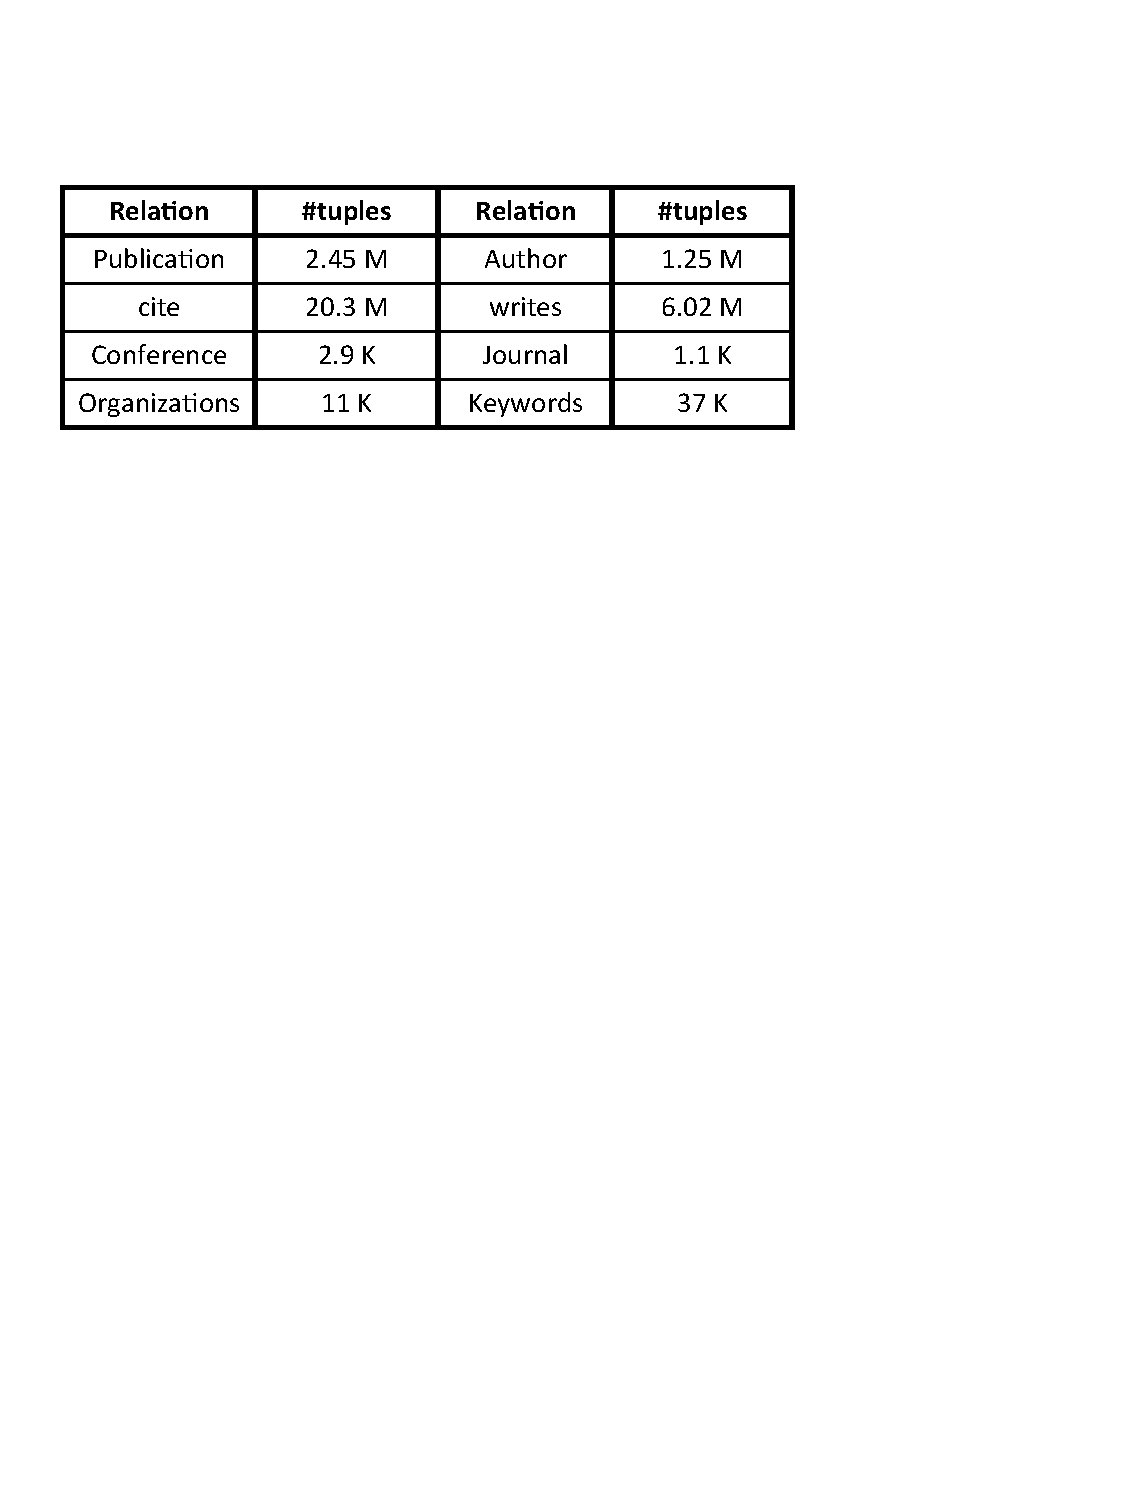
\includegraphics[width=0.8\linewidth]{pic/statistics.pdf}
  \caption{Summary Statistics for MAS Dataset.}
  \label{fig:statistics}
\end{figure}

\subsection{Disambiguation at Entity Level}
\label{subsec:disambiguationEntity}
As mentioned, when mapping the phrases specified by the user to the entities stored in the database, multiple matches might exist and the system need to figure out which ones are the desired.  In our system, two tasks exist.  First, we need to find the best combination of matches for the set of phrases specified in a query.  All matches in this combination are used as the default mapping for each entity.  Second, our system is designed as an interactive system, which returns multiple mappings for each ambiguous entity.  As such, we need to generate a ranked list of matches as alternatives for the user to choose from, which aims to do the entity matching correctly under the help of the user, even in the cases when the default combination of matches is wrong.  Specifically, we generate 5 alternative matches for each entity phrase. 

\paragraph*{Comparisons}
For the task of generating the best match combination, most previous works in graph-based keyword search~\cite{DBLP:conf/icde/BhalotiaHNCS02,DBLP:conf/icde/DingYWQZL07,DBLP:conf/sigmod/GolenbergKS08} just take the match combination in the shortest joining network of tuples.  Our method takes a step further, which considers the combination appears most frequently in all the join networks of tuples within a length threshold.  In the experiments, we compare our strategy with that provided in~\cite{DBLP:conf/sigmod/GolenbergKS08}, in which the match combination in the shortest (with lowest weight) joining network of tuples.  For the task of generating alternative matches for each single entity phrase, previous works often rank the matches based only on the spelling~\cite{DBLP:journals/pvldb/LiJ14}.  In contrast, we take both the spelling and the appearance frequency of each single match into account.  We compare our strategy with that provided in~\cite{DBLP:journals/pvldb/LiJ14} in experiments. 

\paragraph*{Test Set}
Unfortunately, MAS does not make its query history public. Therefore, we created our own test set from 5 PhD students majoring in computer science or information science. All of them have the need to do academic searches and are familiar with many of the famous authors, publications, conferences, journals, organizations, organizations, and hot topics in the subdomain they are focused.  Each of them was asked to specify 5 groups of ambiguous entities.  In a group, each entity are often not easy to be distinguished by itself but can be distinguished when all the entities in the group are considered.  Sample examples are shown in Figure~\ref{fig:sampleEntities}.  Thus we obtained a test set comprising 20 groups of entities.  The number of entities mentioned in these 20 groups is 42.  

\begin{figure}
  \center
  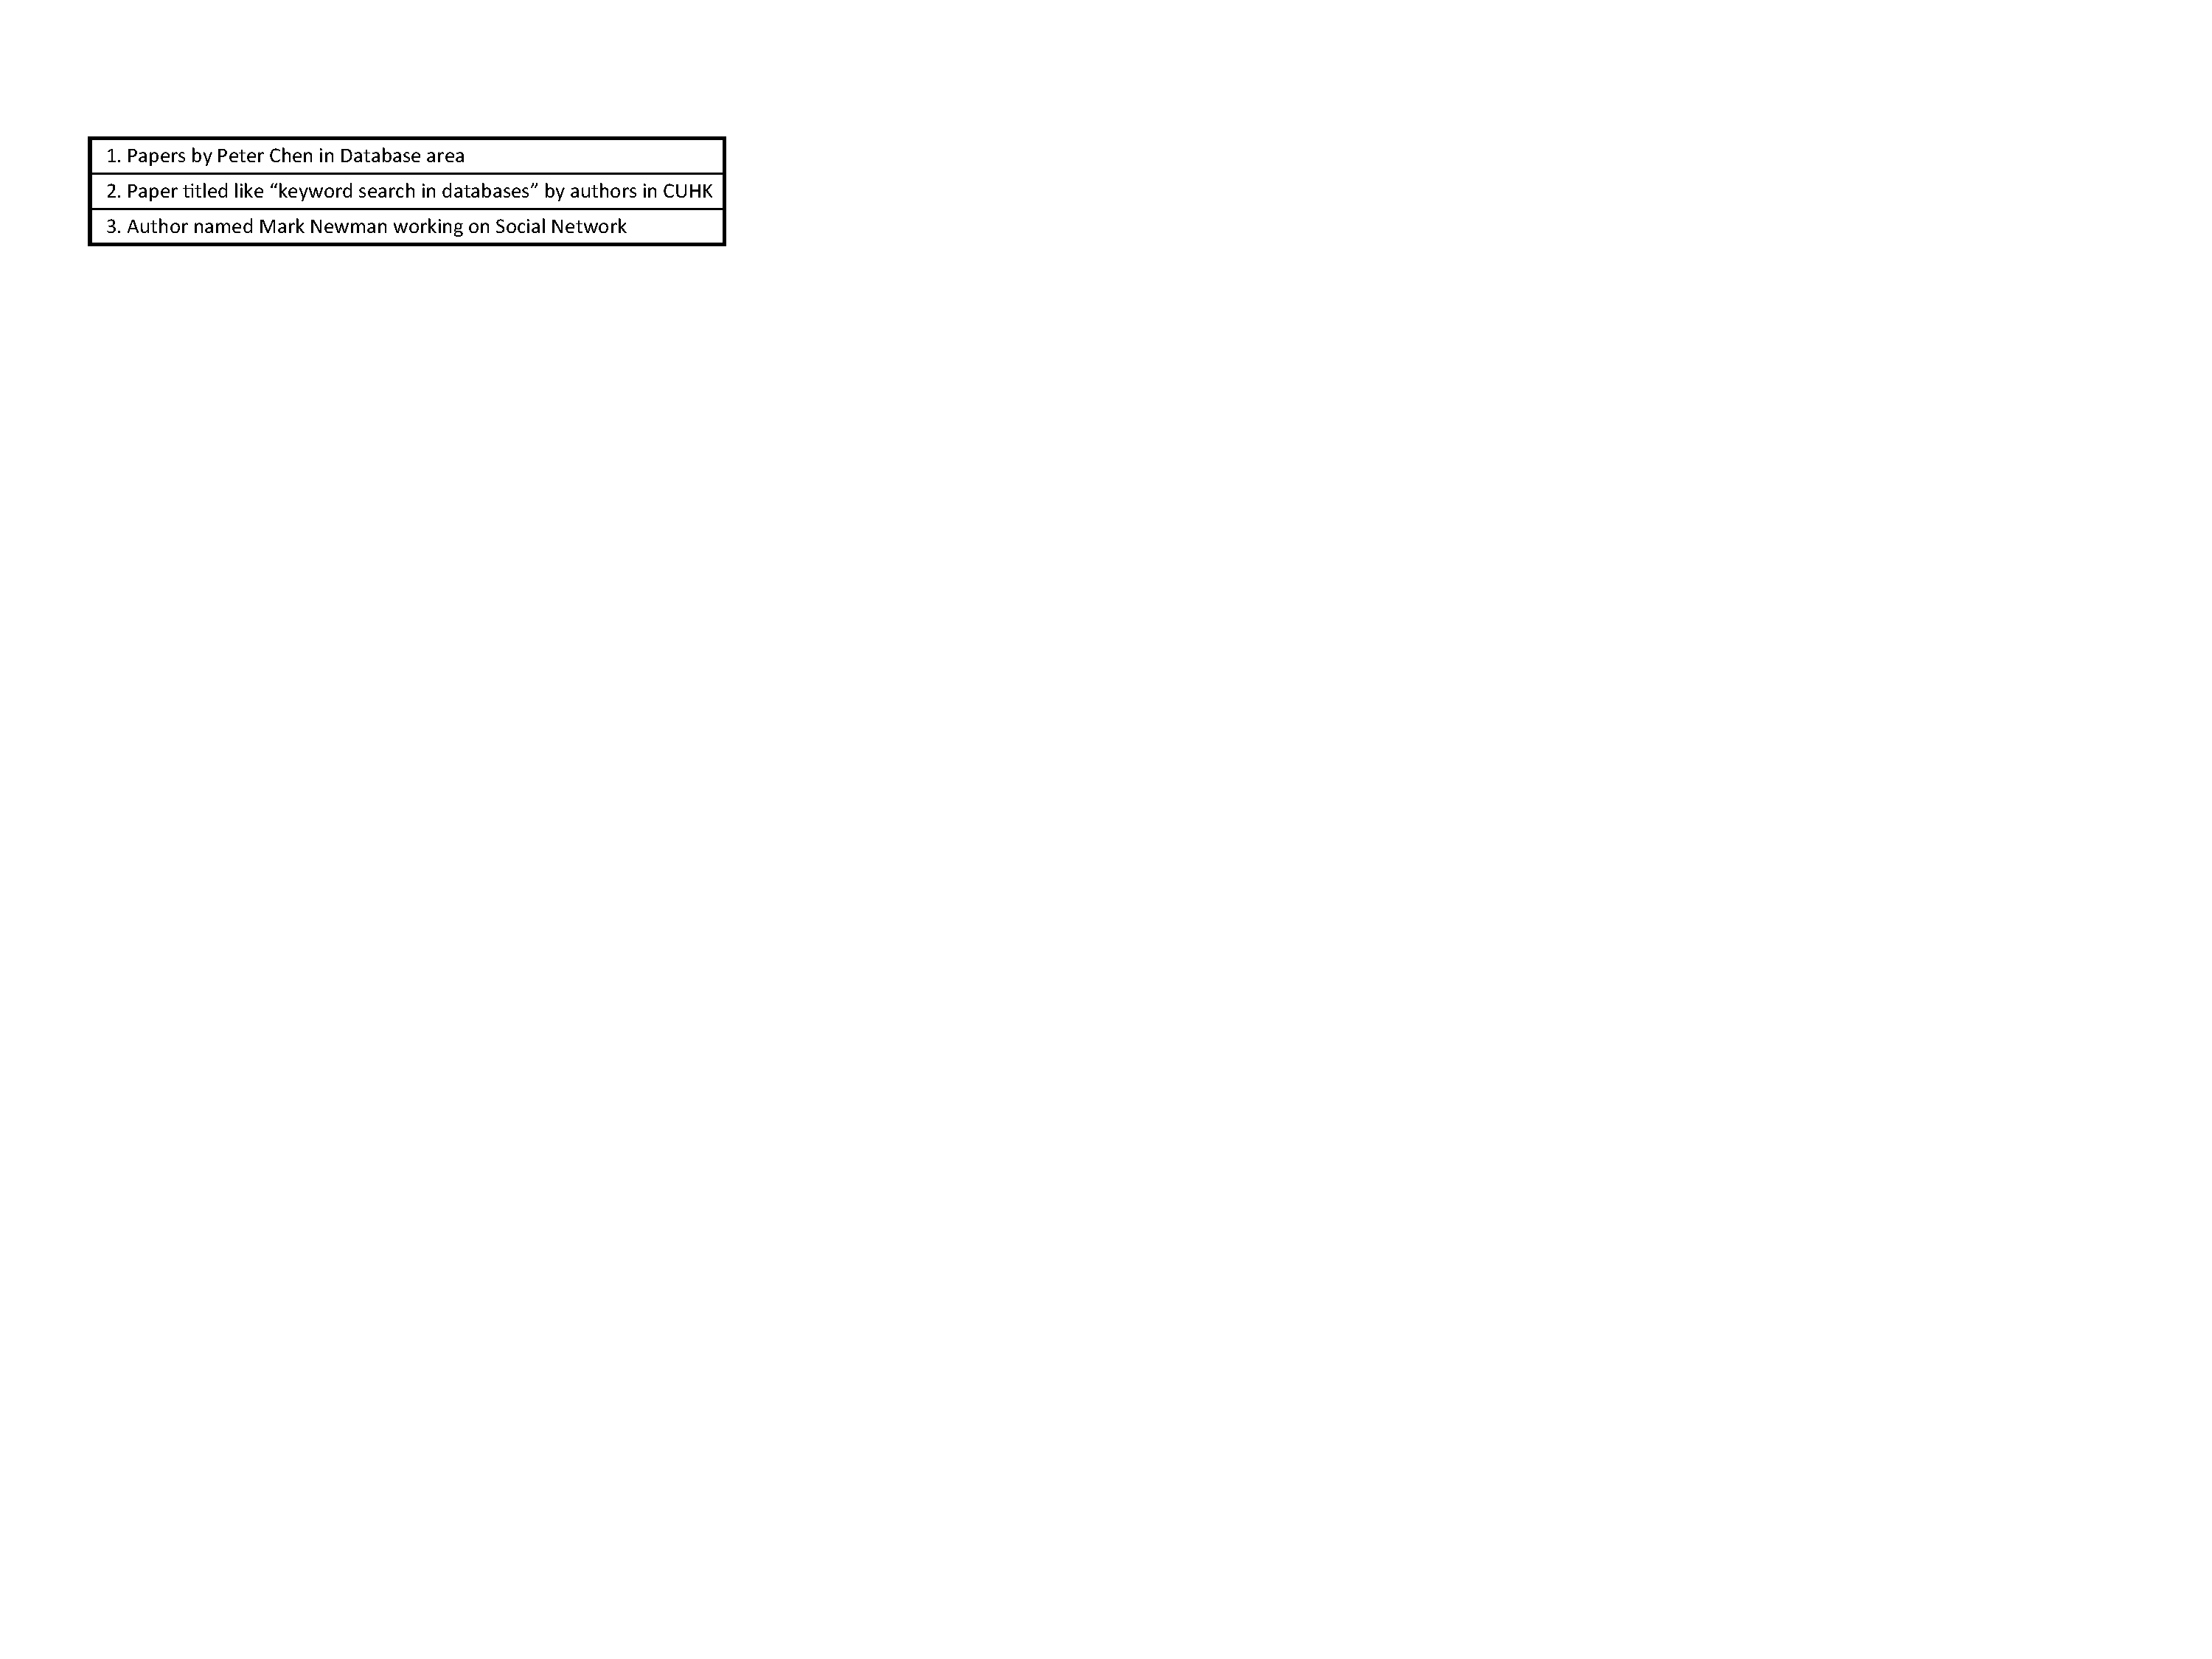
\includegraphics[width=1\linewidth]{pic/sampleEntities.pdf}
  \caption{Samples of Groups of Entities.}
  \label{fig:sampleEntities}
\end{figure}

\paragraph*{Results}
The experimental results for entity disambiguation is shown in Figure~\ref{fig:expEntity}.  For the task of generating the best match combination, the strategy of choosing the match combination in the shortest (with lowest weight) joining network of tuples achieves only a precision of 11/20.  In this strategy, the information in the shortest joining network serves as the only evidence for the matching, which is not often enough to figure out the desired match accurately.  For example, in the first sample group of entities in Figure~\ref{fig:sampleEntities}, the phrase ``Peter Chen" has multiple matches like the Professor who developed the ER model and the Professor in University of Michigan focusing on operation systems and distributed systems.  Both of the two professors have  publications in the database area, which makes it hard to choose the correct one using previous approaches\footnote{Most graph-based keyword search approaches~\cite{DBLP:conf/icde/BhalotiaHNCS02,DBLP:conf/icde/DingYWQZL07,DBLP:conf/sigmod/GolenbergKS08} believe that an edge would carry more information if there are less edges emanated from the node containing the foreign key.  As such, when generating the joining networks of tuples, they prefer to choose the joining network comprising with the nodes having less connections.  However, from our experience and experiments, users are often querying the entities with high connections (famous authors, publications, or conferences).  That would make these approaches work even worse than randomly picking one.  }.  In contrast, when we do the entity disambiguation, we take all the joining networks of tuples into account.  For the first sample group of entities, the Professor who developed the ER model has a much higher combination appearance with the other entity phrase ``database".  As such, our system ranks this combination higher.  

For the individual ranking, our system outperforms the previous strategy significantly.  The reason is that the entities in the test set are all ambiguous ones, in which most of them have many matches that are very similar or even exactly the same with each other.  Also, the specifications of the entity phrases are not often exactly the same with their corresponding entities stored in the database.  As such, the spelling similarity itself is not enough to provide a good ranking.  In our strategy, the relationships between different entities are considered to do the disambiguation, even in the cases when we rank the matches for each single entity phrase.  That helps our system to provide the alternatives accurately in the entity disambiguation process.   

\begin{figure}
  \center
  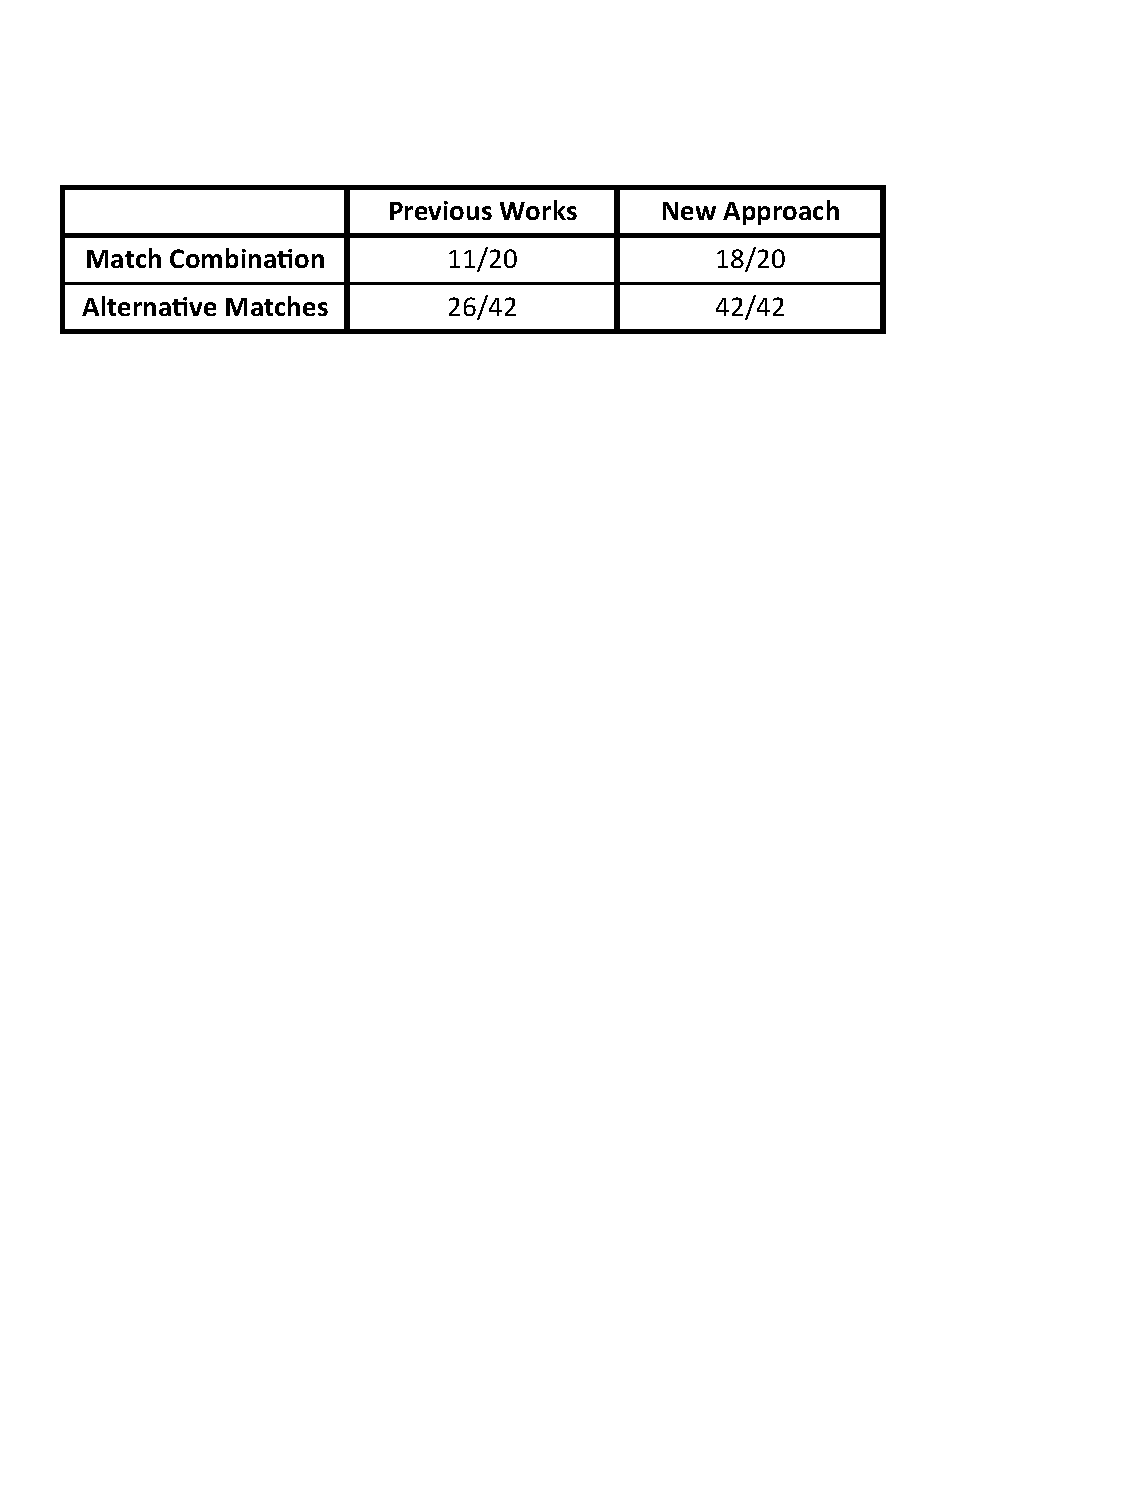
\includegraphics[width=0.95\linewidth]{pic/expEntity.pdf}
  \caption{Entity Disambiguation.}
  \label{fig:expEntity}
\end{figure}

\subsection{Template Mapping}
\label{subsec:disambiguationTemplate}
In our system, the primary step in interpreting a natural language query is mapping it to its desired SQL template.  Specifically, the mapping can be done when no training examples are available and can be improved when training examples are collected.  In this section, we test the effectiveness in the mapping and show the benefits brought from the training examples.  

\paragraph*{Query Task Design}
To test the effectiveness of the mapping process, we need a set of query tasks.  Ideally, these query tasks should cover most of the query logics that are possible to be asked over the database.  To obtain such a set of query tasks, we examine the old version interface of MAS dataset.  It was a carefully designed faceted interface.  By clicking through the site, a user is able to get answers to many quite complex queries.  We enumerated all query logics that are directly supported by the MAS website and obtained a set of 196 SQL templates.  We noticed that the semantic coverage of the MAS website was constrained by the overall design of the interface. As a result, some likely query logics are not supported because they would require a redesign of the interface and impact the overall visual effect. Also, it is possible that some unnecessary query logics are supported just because they are more compatible with interface.  To address these shortcomings, we asked five domain experts, who often do academic searches and have a good sense of which questions would be frequently asked over a bibliographic database, to modify this set of query logics, deleting unnecessary ones and adding new ones as needed.  In this process, we accepted a modification only when it had the agreement of all five experts.  The final set of query tasks $Q_{gold}$ we obtained is composed of 160 different query logics (corresponds to different SQL templates).  Specifically, $Q_{gold}$ contains various kinds of complex queries, in which 110, 52, 53, 34 of their corresponding SQL templates contain aggregations, long join paths with length $\geq$ 5, subqueries, and multilevel of subqueries, respectively.  

\paragraph*{Training Set and Testing Set}
The motivation of our system is to enable users to query the database though natural language. As such, the training set and testing set must be collected from real users. In the collection process, sixteen participants were recruited with flyers posted on a university campus. A questionnaire indicated that all participants were familiar with keyword search interfaces (e.g. Google), but had little knowledge of formal query languages (e.g. SQL). Furthermore, they were fluent in both English and Chinese. For our experiments, it is hard to convey the query task to the participants since any English description would cause bias in the task. To overcome this, we described each query task in Chinese and asked users to compose English query sentences. Since English and Chinese are in entirely different language families and we believe this kind of design can minimize such bias. We transformed each of the query logics into a query task and evenly divided the query tasks into 16 task groups, in which each task group contained 10 query tasks. Each participant randomly took 5 task groups and composed the natural language query according to the Chinese description. After that, we got 800 natural language queries, in which each query logic in $Q_{gold}$ obtained 5 natural language queries.  

For each experiment, we randomly pick one natural language query for each query logic in $Q_{gold}$.  These 160 natural language queries form the testing set.  A subset of the other 640 natural language queries together with their corresponding SQL templates are used as the training set, according to the number of training examples needed.  

\paragraph*{Semantic Coverage}
In our system, the quality of the semantic coverage directly affects the behavior of the online part.  In the experiments, a set of 300 SQL templates are adopted as the semantic coverage, which is automatically generated and contains all the 160 query logics in $Q_{gold}$.  

\paragraph*{Measurements}
We evaluate effectiveness of the top 1 mapping as $|M_P|/|M_T|$, in which $|M_T|$ is the total number of queries and $|M_P|$ is the number of queries that can be mapped to the correct SQL templates in the top 1 mapping.  Remember that our system also returns alternative SQL templates for the user to choose from.  As such, we also evaluate the effectiveness of the top 5 mappings returned as $|M_R|/|M_T|$, in which $M_R$ is the number of queries in which one of the top mappings returned is correct.  Specifically, our system returns the user at most five candidate interpretations.  

\begin{figure}
  \center
  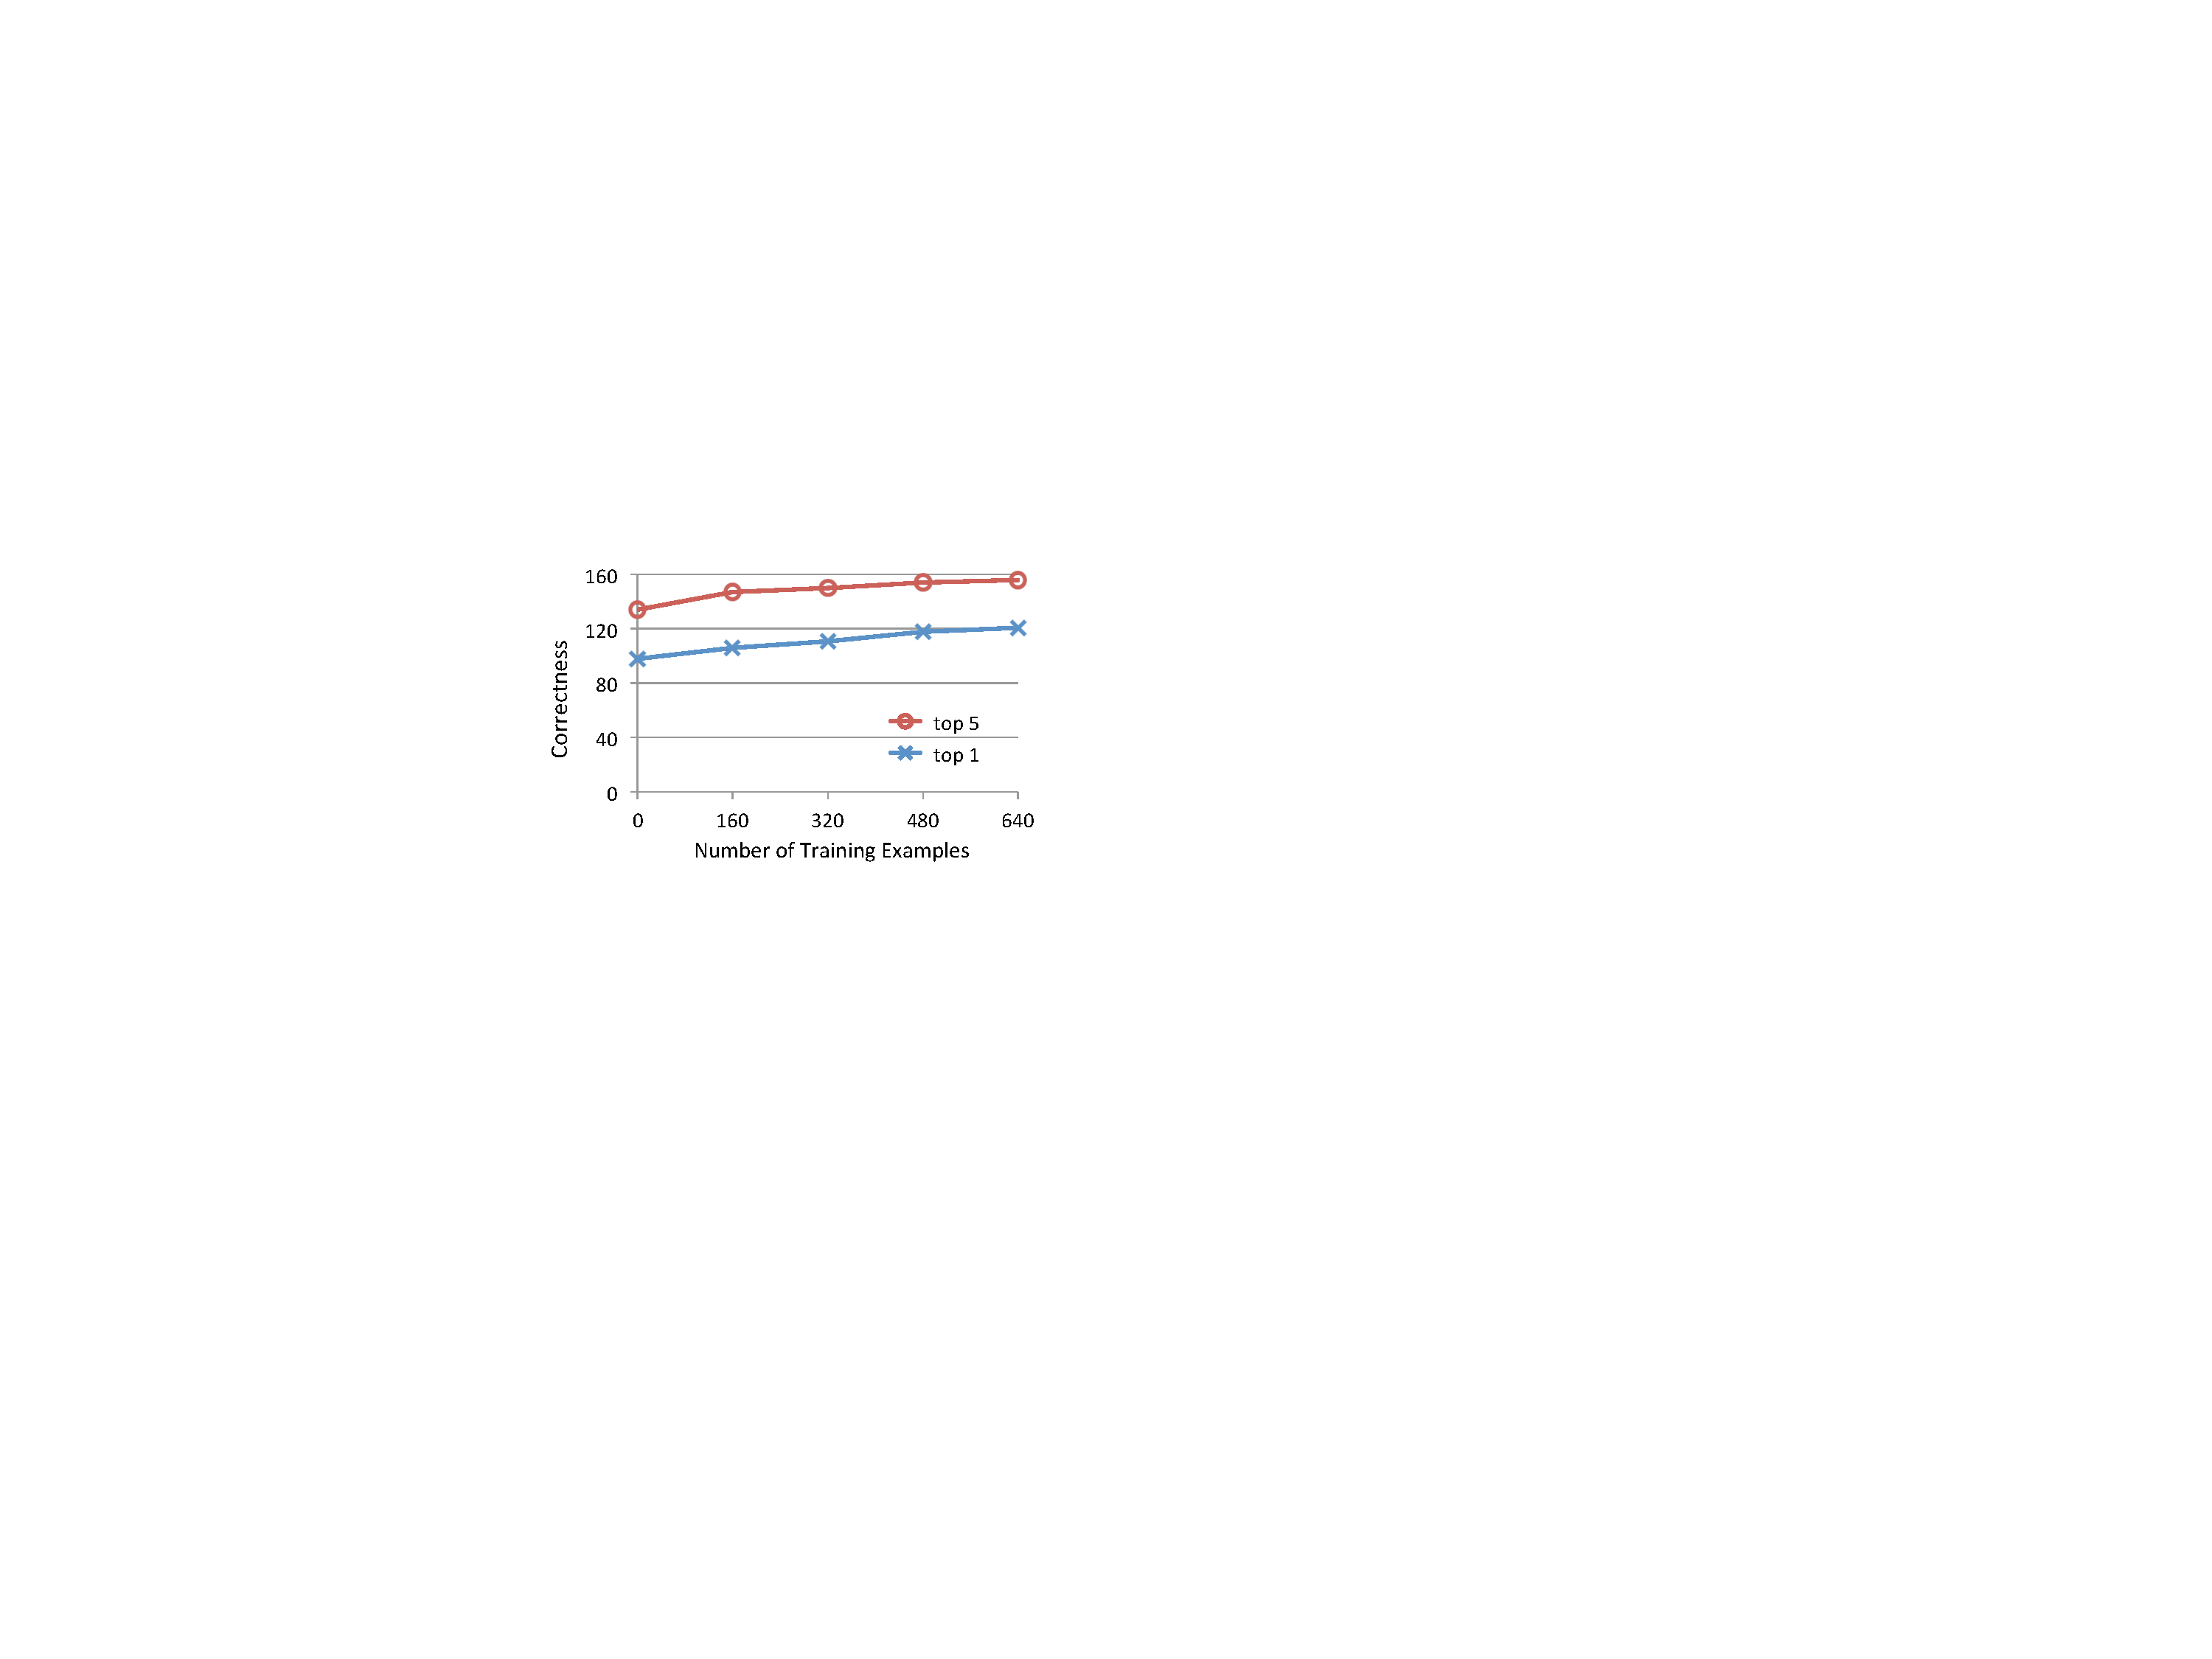
\includegraphics[width=0.75\linewidth]{pic/experimentsTraining}
  \caption{Summary Statistics for MAS Dataset.}
  \label{fig:templateMapping}
\end{figure}

\paragraph*{Results}
The results are shown in Figure~\ref{fig:templateMapping}.  $|M_P|$ grows from 98 to 121 when training examples are added.  $|M_R|$ grows from 134 to 156 with the training examples.  We also compare our system with NaLIR~\cite{DBLP:journals/pvldb/LiJ14} and TBNaLIR.  NaLIR is a generic NLIDB whose semantic coverage is the syntactically valid SQL statements (under some syntactical constraints).  TBNaLIR is a template-based NLIDB, which maps natural language query to the weighted SQL templates using generic metrics.  Specifically, the SQL templates used in TBNaLIR are the same as that used in our system.  Using NaLIR, the $|M_P|$ and $|M_R|$ are 84 and 101, respectively.  For TBNaLIR, the $|M_P|$ and $|M_R|$ are 101 and 135, respectively.  Our method outperform NaLIR and TBNaLIR a lot when training examples are added.  

%=====================Related Work==========================================================
\section{Related Work}
\label{sec:relatedWork}
The problem of constructing Natural Language Interfaces to DataBases (NLIDB) has been studied for several decades.  Early systems often model the problem as a semantic parsing problem, in which grammars are either manually specified~\cite{DBLP:journals/nle/AndroutsopoulosRT95} or learned from training examples~\cite{Zelle:1996:LPD:1864519.1864543,DBLP:conf/ecml/TangM01,DBLP:bibsonomy_ge2005,DBLP:conf/acl/WongM07}.  While quite successful in some specific scenario, the grammars are hard to scale up, both to other domains and to new natural language expressions, which limits the impact~\cite{Liang:2011:LDC:2002472.2002547}.  

In recent years, deep learning methods have achieved great success in machine translation~\cite{DBLP:journals/corr/WuSCLNMKCGMKSJL16} and question answer matching~\cite{DBLP:conf/acl/TanSXZ16,DBLP:conf/cikm/FengXZ16}.  This fact inspires researchers to apply end-to-end frameworks to build NLIDBs~\cite{DBLP:conf/acl/DongL16,DBLP:journals/debu/LuLK16,DBLP:journals/cacm/Liang16,DBLP:journals/tacl/ReddyTCKDSL16}.  From our experience, three major challenges exist in adopting end-to-end framework to construct NLIDBs.  First, the underlying database schema of different NLIDBs often differs, which means the training set used for one NLIDB cannot be applied to another.  As a result, in a real application, it is almost impossible to collect enough pairs of (NLQ, SQL) for an end-to-end model.  Second, as pointed out in~\cite{DBLP:conf/iui/PopescuEK03,DBLP:journals/pvldb/LiJ14}, reliability is very important in database applications.  Users will be very frustrated if they make wrong decisions only because they believe in the wrong results from an NLIDB.  As such, explanations are often necessary for users to understand the processing process.  However, for deep learning methods,  the intermediate structures are often unexplanable.  Third, as discussed in this chapter, NLIDB has many unique resources for resolving ambiguities, like the underlying schema structure, the query log, the distribution of the data, the configuration from the DBA, and so forth.  However, in end-to-end methods, the fact that more resources taken into account often means higher dimensions of input, which would exacerbate the first problem of lacking training examples.  Considering the above obstacles, we develop a new framework instead of simply adopting their methods.  

Another branch of research works focused on building generic NLIDBs~\cite{DBLP:conf/iui/PopescuEK03,DBLP:conf/coling/PopescuAEKY04,DBLP:journals/tods/LiYJ07,DBLP:journals/pvldb/LiJ14} arose as a response to avoid the tedious configuration requirements.  PRECISE~\cite{DBLP:conf/iui/PopescuEK03,DBLP:conf/coling/PopescuAEKY04} defines a subset of natural language queries as semantically tractable queries and precisely translates these queries into corresponding SQL queries.  NaLIX~\cite{DBLP:conf/sigmod/LiYJ05} defines a domain-independent grammar for the natural language queries that are semantically expressible by XQuery and parses natural language queries to XQuery statements according to the grammar.  NaLIR~\cite{DBLP:journals/pvldb/LiJ14} is designed to support complex natural language queries, in which the semantic coverage is defined as all the syntactically valid SQL statements (with some constraints).  By transforming natural language queries to the correct points in the semantic coverage in a series steps, the queries can be translated to the desired SQL statements.  In general, existing generic NLIDBs still define their semantic coverage at the syntax level.  In our system, an offline part is used to refine the semantic coverage, which supports only the query logics that are likely to be queried.  By greatly narrowing down the semantic coverage, the burden in online mapping is reduced.  

From our point of view, the deep learning based methods and generic NLIDBs are taking two extreme strategies.  The deep learning based methods are trying to learn everything from training examples while the generic NLIDBs are avoiding training examples.  We believe that an ideal NLIDB should be provide reasonable results when cold starts and its performance can improve through the usage by collecting the user's behavior.  

Keyword search interfaces are widely used by non-experts to specify ad-hoc queries over relational databases~\cite{DBLP:series/synthesis/2010Yu,DBLP:conf/icde/BhalotiaHNCS02,DBLP:conf/icde/AgrawalCD02,DBLP:conf/vldb/HristidisP02}. Recently, there has been a stream of such research on keyword search~\cite{DBLP:conf/sigmod/TataL08,DBLP:journals/vldb/SimitsisKI08,DBLP:conf/sigmod/ChuBCDN09,DBLP:journals/pvldb/XinHG10,DBLP:conf/icde/FanLZ11,DBLP:journals/pvldb/BlunschiJKMS12,DBLP:journals/pvldb/BergamaschiGILV13}, in which, given a set of keywords, instead of finding the data relevant to these keywords, they try to interpret the query intent behind the keywords in the view of a formal query language. In particular, some of them extend keywords by supporting aggregation functions~\cite{DBLP:conf/sigmod/TataL08}, Boolean operators~\cite{DBLP:journals/vldb/SimitsisKI08}, query language fragments~\cite{DBLP:journals/pvldb/BlunschiJKMS12}, and so forth. These works can be considered as a first step toward addressing the challenge of natural language querying. Our work builds upon this stream of research and supports a richer query mechanism that allows us to convey much more complex semantic meaning than a flat collection of keywords.

The framework of our system is inspired from search engines~\cite{DBLP:journals/cn/BrinP98,Page99thepagerank}.  Similar to NLIDBs, search engines are heuristic query systems, whose queries do not have formally defined semantic meanings. The semantic coverage of a search engine is a large set of webpages.  In the early stage of search engines, search engines maps the keywords to the webpages based on predefined metrics, like the importance of each webpage (e.g. PageRank) and the relevance between the keywords and each webpage (e.g. tf-idf).  After collecting training data, which is in the form of (keyword, webpage clicked), learning to rank frameworks are adopted to improve the quality of the mapping~\cite{DBLP:books/daglib/0027504}.  Inspired from search engines, we model the natural language query interpretation problem as a mapping problem between the natural language query to a point in the semantic coverage.  In this framework, when no training examples are available, predefined metrics are provided to map the input query to the SQL templates.  It also collects training data through the usage and benefits from the training data collected to improve its performance.

The word embedding is a key step in our system.  The method we adopted is word2vec~\cite{DBLP:journals/corr/abs-1301-3781}.  Their model learns a vector representation for each word using a (shallow) neural network language model.  The authors demonstrate that semantic relationships are often preserved in vector operations on word vectors, such as vec(Picasso) - vec(painter) $\approx$ vec(Einstein) - vec(scientist)~\cite{DBLP:conf/nips/MikolovSCCD13}.  Learning the word embedding is entirely unsupervised and it can be computed on the text corpus of interest or be pre-computed in advance. 

One problem in our system is how to evaluate the similarity between sentences.  A stream of research attempts to solve this problem by learning a latent low-dimensional representation of sentences and work well in document matching~\cite{DBLP:conf/icml/LeM14}.  However, this strategy does not work well in our situation, since all the questions over an NLIDB are describing some query logic focusing on a narrow domain (the underlying database).  In such situation, if trained from a generic corpus, the low-dimensional space is not able to distinguish the natural language queries with slightly different query logics.  If trying to train the system from the specific corpus of the NLIDB, collecting enough training examples are still a problem.  So we adopt the general strategy provided in~\cite{DBLP:conf/icml/KusnerGGW15}, which only does the embedding at the word/phrase level.  

Besides the template mapping, the disambiguation at entity level is also a challenge in our system.  One of its similar problem, entity matching, is investigated in the area of data integration and data cleaning~\cite{DBLP:journals/pvldb/GetoorM12}.  Often, manually crafted or learned rules are applied to detect the entities describing the same real world entity between structured data.  In our system, the entity matching is from the entities mentioned in natural language query and the entities stored in the database.  Similar problems are dealt with in graph-based keyword search~\cite{DBLP:conf/icde/BhalotiaHNCS02,DBLP:conf/icde/DingYWQZL07,DBLP:conf/sigmod/GolenbergKS08}, in which the mapped entities in the shortest joining network of tuples are often considered as the best mapping.  In contrast, we provide a principled strategy to compute the probability for each matching.  Both intuitions and experimental results show the improvements over that used in graph-based keyword search.  

A task in our system is to explain the SQL templates for the end users to choose from or for the DBA to fast review.  Previous systems explain SQL queries to users using natural language descriptions~\cite{DBLP:conf/sigmod/KokkalisVZSKI12} or query visualizations~\cite{DBLP:conf/edbt/DanaparamitaG11,DBLP:conf/icde/FanLZ11,DBLP:journals/pvldb/BergamaschiGILV13}.  In our system, we adopt the strategy used in~\cite{DBLP:conf/sigmod/KokkalisVZSKI12}.  

%=====================Conclusions==========================================================
\section{Conclusion and Future Work}
\label{sec:conclusion}

In this paper, we provide a framework for constructing natural language query interfaces over relational databases.  In the framework, the semantic coverage of an NLIDB is defined as a set of SQL templates.  Given a natural language query, by mapping it to the correct SQL template in the semantic coverage, the query can be translated into the desired SQL statement, which may include comparison predicates, conjunctions, quantifications, multi-level aggregations, nestings, and various types of joins, among other things.  In the cases when no training data is available, the mapping is mainly based on the relevance metrics between the natural language query and SQL templates.  When some training examples are obtained, learning to rank is adopted to improve the mapping.  Our system also provide the interactions with the user, which collects the user behavior data as the training set and improve the behavior of our system through the usage.

\bibliographystyle{abbrv}
\bibliography{my-bib-database}
\end{document} 